\chapter{RAN: Reweighting Adversarial Networks}
\label{chap:ran}
\section{The need for full spectral measurements.}
    \label{sec:need-for-density-unfolding}
    \subsection{Motivation: beyond moments and binned spectra.}
    Measurements in high energy physics traditionally report differential cross sections in a binned format, or even just a few summary statistics (moments) of a distribution. 
    %
    This approach has produced numerous important results in the past~\cite{GomezAmbrosio:2022mpm, Benato:2025rgo, ATLAS:2017dhr, alhroobSingleTopQuark,cowan_statistical_1998}, but it fundamentally limits the information available for theoretical interpretation.
    %
    A small set of moments offers only a coarse summary of a probability distribution and can hide critical features.
    %
    In fact, infinitely many different distributions can share the same first few moments.
    %
    Two observables with identical mean and variance may have drastically different tails or multi--modal structures that only a full distribution reveal.
    %
    Thus, relying solely on low order moments risks missing new physics signals or subtle QCD effects that manifest as shape differences rather than overall normalisation changes.

    Binning an observable into histograms is a more detailed approach than just quoting moments, but it too imposes significant limitations.
    %
    Finite bin widths smear out fine structures and impose an arbitrary discretisation on inherently continuous spectra.
    %
    Moreover, once data are binned, it becomes impossible to reconstruct or analyse the distribution for any arbitrary transformation of that observable without returning to the original unbinned data.
    %
    For example, if a cross section is unfolded in bins of an angle $\theta$, one cannot later obtain the distribution in $\cos\theta$ or $\ln\theta$ except by repeating the unfolding from scratch.
    %
    In contrast, an unbinned, ``full spectral,'' measurement preserves maximum information, allowing \textit{a posteriori} reprocessing such as deriving moments, binning into different intervals, or studying functions of the measured observable.
    %
    This flexibility is especially valuable when comparing with various theoretical models, each of which may suggest different variables or summary statistics to highlight.

    Another motivation for capturing the \emph{full differential spectrum} is that many theoretical predictions in quantum chromodynamics (QCD) and beyond are sensitive to the detailed shape of distributions.
    %
    New physics might appear as excess events in the tails of kinematic distributions, or subtle distortions across a spectrum rather than an overall rate change.
    %
    Precision QCD studies often rely on the \emph{scaling patterns} of entire distributions with energy or other parameters, not just their averages.
    %
    By measuring the full spectrum, experimental results can be directly fed into global fits or theory calculations that integrate over the entire phase space.
    %
    In summary, to fully exploit the data and enable the broadest possible comparisons to theory, it is imperative to go beyond a few moments or fixed bin histograms and aim to unfold the continuous differential cross section itself.

    The reminder of the this section discusses some of the central limitations of binned approaches and approaches focused on unfolding a few moments introduced above in greater detail.
    \begin{itemize}
        \item \textbf{Information loss.}
            Low order moments condense an entire distribution into a small handful of numbers.
            %
            This sacrifices information about higher order fluctuations and tail behavior.
            %
            Many distinct distributions can reproduce the same set of moments, so important differences\footnote{e.g. a long tail vs. a sharp cutoff} remain hidden if only moments are reported.
            %
            Even in cases where theory predicts moments more readily than spectra\footnote{as in some QCD calculations of energy scaling of moments}, relying exclusively on moments means discarding data that could otherwise constrain models.
            %
            Binned histograms similarly integrate the underlying distribution over each bin, blurring details smaller than the bin width.
            %
            Fine binning could, in principle, mitigate this, but the detector resolution and statistical limits one's ability to use bins that are too fine.
            %
            Too fine bins lead to instability due to bin migration effects and large uncertainties~\cite{Bessner:2017trm, LHCb:2023qav, ATLAS:2024hmk, CMS:2025dnx, Kutz:2024eaq, ATLAS:2016vlf}.
        \item \textbf{Binning artifacts and biases.}
            Any choice of bin boundaries is inherently arbitrary.
            %
            Two experiments measuring the same observable might choose different binning schemes, complicating direct comparisons.
            %
            Small shifts in bin edges can redistribute events and lead to apparent differences that are purely due to binning choices rather than physics.
            %
            Furthermore, when binning multivariate data\footnote{or examining an observable's moments in bins of another quantity}, the necessary discretisation in each dimension can introduce artificial discontinuities~\cite{GomezAmbrosio:2022mpm, Fiorendi:2014klw, KLOE-2:2025ggc, Ressegotti:2024szk, LHCb:2025eyf, Grosso:2024nho,}.
            %
            These artifacts hinder comparing unfolded results with continuous theoretical predictions or with results from other experiments that used different bin definitions~\cite{Brehmer:2018hga}.
            
            Additionally, binning can bias downstream analysis;
            %
            for instance, extracting moments from a binned distribution requires assuming a shape within each bin~\footnote{often a constant or linear interpolation}.
            %
            If the true distribution varies non--linearly inside the bin, the extracted moment is biased by the bin size and shape assumption such that even the sign of the error cannot be known \textit{a priori}~\cite{desai2024moment}.
            %
            An unbinned measurement eliminates this intermediate step and the bias that can arise from it.
        \item \textbf{Limited dimensionality.}
            Perhaps most importantly, binned unfolding severely constrains the number of observables one can unfold simultaneously.
            %
            Each additional dimension (feature) requires exponentially more bins to maintain a given resolution.
            %
            In practice, traditional unfolding is often performed in just one or two dimensions at a time because higher dimensional histograms would be too sparsely populated.
            %
            This precludes measuring cross sections differential in many variables at once.
            %
            It also means that if one is interested in an observable $O$ that is a complicated function of several kinematic quantities, one either must unfold those quantities jointly with fine binning (which is infeasible) or settle for unfolding a projection of $O$ in one dimension (which loses information).
            %
            In contrast, unbinned approaches can handle high dimensional data naturally, since they do not require constructing an \(d-\)dimensional grid of bins.
            %
            Unfolding the full phase space~\footnote{i.e. a fully differential cross section in all relevant kinematic variables} is only realistic with an unbinned strategy.
    \end{itemize}        

\begin{table}
    \label{tab:meas_compare}
    \centering
    \caption{Comparison of measurement approaches.
    %
    Reporting only low--order moments loses most distribution information.
    %
    Binned differential cross sections retain shape information but suffer from discretization and limited dimensionality.
    %
    Full spectral measurements preserve the complete distribution, enabling maximal reusability and detailed theory comparisons, but require regularizing a much more ill--posed training.
    }
    \begin{tabular}{lccc}
        \toprule
        \textbf{Aspect} & \textbf{Moments only} & \textbf{Binned spectrum} & \textbf{Full spectrum} \\
        \midrule
        Information           & Low   & Moderate & High \\
        Reuse         & High      & Limited  & High \\
        Dimensions    & Many       & 1 to 2   & Many \\
        Stability              & Easy & Moderate & Hard \\
        \bottomrule
    \end{tabular}
\end{table}

    Table~\ref{tab:meas_compare} summarizes these differences between unbinned moment based unfolding, binned density unfolding, and unbinned full spectrum unfolding methods.
    %
    By construction, a full spectral measurement retains maximal information and avoids discretisation issues, at the cost of a more challenging unfolding procedure.
    %
    These challenges were a major deterrent historically, explaining why experiments long favoured simplified results despite their limitations.
    
    \subsection{Use cases.}
    Some of the most compelling motivations for unbinned unfolding of probability density functions come from specific classes of observables and analyses in high energy physics that demand detailed distributions rather than summary measures.
    %
    A few examples are
    \begin{itemize}
        \item \textbf{Jet substructure observables.}
            %
            Modern studies of jet physics often examine intricate internal properties of jets, for example, the distribution of jet mass, angularity, $N-$subjettiness ratios like $\tau_{21}$, energy correlation functions, and so on.
            %
            These observables have rich distributions shaped by QCD radiation and hadronisation inside the jet.
            %
            For instance, the jet mass spectrum in hadronic collisions exhibits a steeply falling shape with resonance peaks or grooming induced features in certain regions;
            %
            capturing these details is essential for validating parton shower models and grooming techniques.
            
            If only the average jet mass or a few quantiles were reported, one would lose the structural information of how often jets are heavy versus light, or how substructure sculpts the distribution.
            %
            Similarly, distributions of $\tau_{21}$ \footnote{a ratio used to tag two prong substructure} contain information about the fraction of jets with two subjets versus one, which is crucial for signal (e.g. boosted $W$) vs background (QCD jet) discrimination.
            %
            Capturing the entire $\tau_{21}$ spectrum allows experimentalists and theorists to identify where in the distribution their models agree or fail, rather than just comparing an efficiency at a fixed cut.
            
            Unfolding these jet substructure distributions in an unbinned way provides a high resolution view of QCD dynamics and is increasingly necessary as theory tools\footnote{like analytic resummation or first principles simulation} improve to the point of predicting differential shapes~\cite{Canelli:2025ybb, H1:2021wkz, Shmakov:2024gkd}.
            %
            In fact, recent measurements have demonstrated the power of full phase space unfolding for jets, using multivariate ML techniques to correct detector effects and obtain particle level jet observable spectra without binning~\cite{Arratia:2021otl, Milton:2025mug,collaboration_machine_2024, collaboration_machine_2025, Aguilar-Saavedra:2014kpa}.
            %
            These cases underscore that jet physics benefits enormously from preserving the full shape information.
        \item \textbf{Charge and flavour sensitive observables.}
            %
            Some observables aim to distinguish particle charge or flavour inside complex final states, and their distributions can be especially telling.
            %
            An example is the jet charge distribution, the electric charge of a jet computed from the momentum weighted charges of its constituent particles.
            %
            This quantity is used to tag whether a jet originated from a quark of a given electric charge\footnote{as opposed to a gluon, which has none}.
            %
            The jet charge is a continuous valued observable that can take positive and negative values, and experiments measure its probability distribution for jets of various momenta.
            %
            The full shape of the jet charge distribution contains information about the underlying quark/gluon mixture and fragmentation processes;
            %
            for instance, a broader distribution indicates a mix of high charge (quark origin) and zero charge (gluon origin) jets, whereas a narrow distribution peaked near zero suggests predominantly gluon jets.
            %
            Only by unfolding the entire jet charge spectrum (including its dependence on jet $p_T$) can one provide data precise enough to tune fragmentation models and compare to theoretical calculations of charge transport in jets~\cite{CMS:2017yer,CMS:2020plq,Larkoski:2024uoc,Accardi:2022oog,Baldenegro:2024pfb,AbdulKhalek:2021gbh, Larkoski2020JetLearning}.
            
            Another example is the distribution of identified particle multiplicities.\footnote{E.g., number of charged hadrons in an event or in a jet}
            %
            The multiplicity distribution is discrete but often measured as a histogram.
            %
            It is a particularly challenging observable to unfold because it is strongly sensitive to soft QCD and hadronization effects~\cite{Lyons:2011cli, Grosse-Oetringhaus:2009eis, ALICE:2022xip, Segura:2024srj, STAR:2022etb, Carli:2015qta, Skands:2014pea, Christiansen:2015yqa}.
            %
            Two Monte Carlo generators might predict the same average multiplicity but differ in the width or tail of the multiplicity distribution, which affects extreme cases.\footnote{Like very high multiplicity events.}
            %
            Such observables are often \emph{infrared unsafe} theoretically,\footnote{because soft particle emission has no cutoff, perturbative predictions diverge for the distribution shape} meaning theory must rely on phenomenological models.
            %
            The only way to constrain and improve those models is for experiments to provide the unfolded full distributions of these IR unsafe observables at particle level.
            %
            In summary, any analysis where internal structure, charge assignments, or other detailed event properties matter will benefit from (or even require) full spectral unfolding rather than a few summary numbers.
        \item \textbf{Multidifferential and high dimensional measurements.}
            The ultimate form of ``full'' spectral measurement is unfolding in multiple kinematic dimensions simultaneously, effectively measuring a multi differential cross section over a high dimensional phase space.
            %
            While this is extremely challenging, certain physics questions demand correlating several observables.
            %
            For example, consider measuring an observable $O$ as a function of another variable (or collection of variables) $\vb{Q}$\footnote{say, the distribution of jet charge $q$ in bins of jet $p_T$ or event energy $Q$}.
            %
            With traditional methods, one would perform a two dimensional unfolding, choosing a projection of \(Q\) if needed (bins in $O$ vs bins in $Q$) to then extract moments or other features as a function of $Q$~\cite{CMS:2011xqa, ATLAS:2010jvh, ATLAS:2020ccu, CMS:2014eaj, ATLAS:2022zbu, DAgostini:265717}.
            %
            Binning in two (or more) dimensions quickly suffers from sparse data in many bins and complicated systematic uncertainties.
            %
            An unbinned approach, by contrast, could in principle unfold the joint $(O,\vb{Q})$ distribution without requiring an explicit grid, allowing arbitrary slicing and analysis after the fact.
            %
            This is especially relevant in the era of high luminosity colliders, where huge datasets invite more differential measurements.
            %
            Rather than publish dozens of separate one dimensional spectra (each in a single kinematic region), one could publish a multi dimensional unfolded distribution that coherently captures all correlations.
            %
            Such a result would be far more powerful for global interpretations, albeit significantly more complex to obtain.
            %
            Unbinned density unfolding techniques are a step toward this ambitious goal, enabling higher dimensional unfolding than previously feasible with manageable uncertainties.
    \end{itemize}
    \subsection{Challenges in unfolding full distributions.}
        The push for unbinned, high resolution unfolded spectra comes with substantial challenges.
        %
        Unfolding a full distribution, especially in multiple dimensions, is a markedly more ill posed problem than unfolding a small set of summary statistics or coarse bins.
        %
        These challenges are statistical, physical, and computational.

        At its core, unfolding requires inverting the detector response---a many to many mapping where a given particle level distribution can produce a range of detector level outcomes due to resolution and inefficiencies.
        %
        This inversion is ill posed, that is to say, infinitely many particle level spectra are, in principle, consistent, within uncertainties, with a given set of detector level data, especially if the data are treated in fine detail.
        %
        Small fluctuations or statistical noise in the detector level histogram can cause huge oscillations in the naive unfolded solution if one attempts a direct inversion of the response matrix.
        %
        In classical unfolding methods, this is well known.
        %
        Directly inverting the response matrix $\mathbf{R}$ leads to amplified noise and unstable solutions.
        %
        The problem is exacerbated when the ``matrix'' is essentially continuous (unbinned) since here one is trying to reconstruct a function rather than a finite vector, which has infinitely many degrees of freedom.
        %
        Without any constraints or regularisation, unfolding is mathematically underdetermined; one must introduce additional information to obtain a physical solution.
        %
        This additional information can be statistical regularisation\footnote{E.g., penalizing roughness in the solution}, or a strong prior\footnote{Incorporated, e.g., initial guess of the spectrum} to guide the result.
        %
        Either way, the unfolded distribution will depend to some degree on these assumptions, which is a point of concern.

        All unfolding methods require some initial model or ansatz for the true distribution, explicitly or implicitly.
        %
        Traditional regularised unfolding (e.g. Bayesian iterative methods or Tikhonov regularisation) starts from a prior distribution and updates it in light of the data.
        %
        If the prior is significantly wrong in a region where data have low sensitivity, the unfolded result may inherit that wrong shape (bias) because there isn't enough information in the data to correct it.
        %
        For binned methods with strong regularisation, the unfolded spectrum can end up looking very much like the prior except in regions where the data clearly indicate otherwise.
        %
        When unfolding a full spectrum, prior dependence can be even trickier.
        
        With many bins or continuous degrees of freedom, there are more opportunities for the prior assumptions to creep in unless the method explicitly works to mitigate this.
        %
        Modern ML based unbinned unfolding techniques like iterative reweighting (used by {\textsc{OmniFold}) attempt to reduce prior bias by gradually adjusting the prior to fit the data, but they still require that the initial simulation populate all regions of phase space that data might cover.
        %
        In other words, if the Truth has support outside the domain of the Generation, no unfolding can recover that---a condition that applies to all known methods.
        %
        This need for sufficient overlap in the support of the prior and true distributions is a fundamental mathematical limitation: full spectral unfolding demands that our Generation model is flexible and broad enough to encompass the Truth, at least roughly, or else certain features will be missed entirely.
        %
        Methods such as \textsc{OmniFold} that involve classification and reweighting at detector level in addition to particle level additionally require that Simulation populate the entire phase space of Data.

        Unfolding more finely, or in more dimensions, inherently means extracting more parameters.\footnote{In effect, more bins worth of information.} from the same finite dataset.
        %
        This trade off means individual elements of the unfolded spectrum will have larger statistical uncertainties than if the data were aggregated into a few bins or moments.
        %
        For example, unfolding 100 bins will yield each bin count with larger uncertainty than if one had combined them into 10 bins.
        %
        If not carefully handled, an unbinned unfolding will overfit statistical fluctuations in the observed data.\footnote{Referred to as \emph{sculpting} in the machine learning literature~\cite{Corso2023, ParticleDataGroup:2022pth}.}
        %
        Effective regularisation is essential to prevent noise amplification.
        
        Additionally, the detector response kernel must be well modelled.
        %
        Any mismodeling (systematic error) will imprint itself on the unfolded result in complex and unpredictable ways.
        %
        When only a few numbers are extracted, one can sometimes correct for known detector biases by simple scale factors; but when unfolding an entire distribution, any mismodeling of the response shape can distort the unfolded spectrum non-uniformly.
        %
        This places high demands on detector simulation fidelity and on methods to incorporate systematic uncertainties (e.g. variations of the response model) into the unfolding procedure.
        %
        Fully Bayesian approaches or profile likelihood methods can propagate uncertainties to the unfolded spectrum, but doing so in high dimensions is computationally intensive.
        %
        In short, the richer the information one unfolds, the more careful one must be to quantify the reliability of each feature of the spectrum.

        Traditional unfolding algorithms scale poorly as the number of bins grows.
        %
        Even if one had infinite amounts of data and so unpopulated bins were not a concern, these traditional algorithms like iterative Bayesian unfolding (IBU, or the D'Agostini method) that are relatively fast for tens of bins become very slow for hundreds of bins, and practically unusable for thousands of bins or continuous data, as each iteration must refine a fine grained distribution.
        %
        Unbinned algorithms, on the other hand, typically rely on machine learning or Monte Carlo sampling.
        %
        They may involve training complex models on large datasets or performing high dimensional optimisations.
        %
        For instance, iterative reweighting methods train a classifier multiple times\footnote{Each iteration is a full supervised learning task on the dataset}, and generative approaches might require training a high capacity generative model on millions of events.
        %
        These computations require substantial computing resources (CPU and GPU), careful hyperparameter tuning, and sometimes suffer from convergence issues.
        %
        Ensuring that an unbinned unfolding converges to a stable solution without excessive computation is a non-trivial challenge.
        %
        In summary, the practical feasibility of unfolding full spectra depends on advances in algorithms and computing, precisely the advances that modern machine learning based methods aim to provide.
        
        Despite the challenges that unfolding full spectra presents, the drive to measure full spectra is strong because of the scientific payoff.
        %
        The next subsection discusses how recent machine learning methods, including the RAN architecture, tackle these issues.

    \subsection{Unbinned unfolding approaches.}
        Recent years have seen rapid development of machine learning techniques for unfolding, which seek to overcome the limitations of traditional methods and make full spectral measurements possible in practice.
        %
        Broadly, these approaches fall into two categories, those based on \textit{reweighting} an existing simulated sample to better agree with data, and those based on \textit{generating} new events\footnote{Typically with generative models.} to reproduce the data distribution.
        %
        Both categories strive to avoid fixed histogram binning and instead work with unbinned data, using the power of ML to handle high dimensional inputs and complex detector responses.

        One of the pioneering ML based methods is \emph{\textsc{OmniFold}}, which introduced an unbinned, multivariate unfolding technique using iterative reweighting.
        %
        {\textsc{OmniFold} uses classifier neural networks to reweight a Monte Carlo sample.
        %
        Essentially, it trains classifiers to distinguish between data and simulation, and then uses the classifier output to assign weights to simulation events such that the weighted simulation better matches the data.
        %
        This procedure is done in stages (iterations) and at both detector and particle level in alternation.
        %
        The method produces a set of weights for Generation events that yield an unfolded distribution.
        %
        \textsc{OmniFold} demonstrated, for the first time, that one can simultaneously unfold many observables\footnote{And even the entire event record.} without binning, given a sufficiently flexible classifier and a robust iterative scheme.
        %
        It has been successfully applied in multiple experimental analyses.
        
        The key advantages of \textsc{OmniFold} are that it naturally accounts for high dimensional correlations\footnote{Since the classifier can use any or all features} and it actively mitigates prior dependence by iterative refinement, effectively performing a form of expectation maximisation to find a self consistent unfolded result that does not overly rely on the initial generation distribution.
        %
        However, a noted downside is its computational cost: each iteration requires training two classifiers to convergence, and in realistic cases one might need $\numrange{5}{10}$ iterations, amounting to training a large number of networks.
        %
        This iterative nature can also complicate uncertainty evaluation and hyperparameter tuning.\footnote{E.g., one must subjectively choose when to stop iterating to avoid instability.}
        %
        Still, \textsc{OmniFold} set the stage for practical unbinned unfolding and proved the feasibility of full spectral measurements on real collider data.

        In parallel, other methods have explored using explicit generative models to unfold distributions.
        %
        For example, VAEs have been employed to learn a mapping from random noise to particle level distributions such that, when those events are passed through a detector simulation, the output matches the observed data distribution.
        %
        Similarly, normalising flows and other invertible neural networks have been used to model the probability density function of true observables and deform it until its convolution with the detector response matches data.
        %
        These approaches are extremely powerful in principle: a sufficiently flexible generator could capture the full true distribution without needing a starting simulation.
        %
        In practice, however, training such generative models is challenging.
        %
        Pure generative unfolding would require vast amounts of data to constrain the high dimensional space and can suffer from mode dropping.\footnote{The generator might fail to produce some less common features of the distribution if not properly incentivised.}
        %
        Additionally, learning a full generative model from scratch means the method must learn \emph{both} the underlying physics distribution \emph{and} compensate for detector effects at the same time.
        %
        This is a high dimensional optimisation that can be unstable or require careful conditioning.
        %
        Some recent works have attempted to combine generative modelling with explicit usage of the known detector response to guide the training\footnote{For instance, by using differentiable detectors or gradient-based deconvolution}, but these are still at the experimental stage.

        Between pure reweighting (which uses an existing simulation as a starting point) and pure generation (which starts from random noise) lies an attractive compromise: using machine learning to \emph{reweight or recalibrate} an initial simulation in a single pass, by directly comparing its predictions to data.
        %
        The \textbf{Reweighting Adversarial Networks (RAN)} method is built on this approach.
        %
        Other examples include optimal transport inspired methods that train a single neural network to learn a transport map by minimising some distance between weighted simulation and data distributions.
        %
        Such approaches leverage the fact that modern simulations are a good but imperfect approximation of reality; rather than throw them away and learn from scratch, it may be easier to learn small corrections (reweightings) to the simulation.
        %
        In this sense, RAN and similar methods treat unfolding as a density ratio estimation problem: find a function $g(z)$ such that the weighted MC distribution $g(z)\,q(z)$ matches the true distribution $p(z)$.
        %
        If $Z$ denotes particle level kinematics, this $g(z)$ effectively encapsulates how the Monte Carlo needs to be modified to agree with nature.
        
        The challenge is that we cannot observe $p(z)$ directly---we only have access to its smeared version at detector level.
        %
        Therefore, these algorithms set up a two level training objective to adjust $g(z)$ based on how well the weighted events, after going through the detector simulation, agree with the detector level data.
        %
        This two level problem is naturally addressed with adversarial setups that train a simulator or reweightor function in competition with a discriminator, or with optimal transport objectives that connect particle and detector level distributions.

        In summary, the landscape of modern unfolding methods includes iterative classifiers (\textsc{OmniFold}), single shot adversarial reweighting (e.g. RAN), and generative approaches (cINNs, VAEs), each with their own strengths.
        %
        \cref{tab:unfold_methods} provides a high level comparison.
        %
        All these methods aim to enable unbinned, high dimensional unfolding; they chiefly differ in how they incorporate prior knowledge, whether they iterate, and how computationally intensive they are.
        %
        Notably, most current ML based methods still require that the starting simulation has support in the regions of interest.
        %
        They also share common challenges of training stability and overfitting prevention, which are addressed through techniques like regularisation or specific loss functions.\footnote{For instance, \textsc{OmniFold} uses early stopping of iterations, while adversarial methods use regularised neural network architectural constraints.}

         \begin{table}
            \centering
            \caption[Comparison of unfolding method characteristics]{Comparison of key characteristics across different unfolding methods. ``Unbinned'' indicates whether the method can process continuous data without binning into fixed histograms. ``Iterative'' refers to whether multiple training iterations are required (distinct from neural network training epochs). ``Uses simulation'' indicates whether the method reweights existing Monte Carlo events (Yes) or generates new samples from scratch (No). The Reweighting Adversarial Network (RAN) method introduced in this chapter combines the advantages of unbinned processing and non-iterative training while leveraging prior simulations, positioning it between the computational efficiency of traditional methods and the flexibility of modern machine learning approaches.}
            \label{tab:unfold_methods}
            \begin{tabular}{lccc}
                \toprule
                \textbf{Method} & \textbf{Unbinned} & \textbf{Iterative} & \textbf{Uses sim.} \\
                \midrule
                Traditional (IBU, TUnfold) & No & Sometimes & Yes\\
                Discriminative (\textsc{OmniFold})      & Yes & Yes & Yes \\
                Generative (cINNs/VAEs)             & Yes & No  & No (from noise)\\
                Adversarial reweight (RAN)        & Yes & No  & Yes \\
                \bottomrule
            \end{tabular}
        \end{table}

    \subsection{Addressing challenges.}
        The Reweighting Adversarial Networks (RAN) approach described in this chapter is designed to tackle the aforementioned challenges head on, enabling full spectral unfolding with improved stability and efficiency.
        %
        This section outlines how the methodology of RAN addresses the needs and difficulties detailed above.\footnote{A complete description of the method follows in later sections, so the focus here is on concepts rather than implementation details.}
        
        RAN explicitly targets the entire distribution rather than a fixed set of moments.
        %
        In fact, it can be viewed as an extension of the Moment Unfolding method described in \cref{chap:moment-unfolding} to infinitely many moments.
        %
        By using a flexible neural network to parametrise the weighting function, RAN does not impose a rigid functional form limited to a few moment constraints.
        %
        This means it has the capacity to adjust the simulation such that not only the first few moments.
        %
        \emph{All} features of the distribution\footnote{In principle, every differential element.} are brought into agreement with the observed data.
        %
        Framing the problem this way ensures that when RAN converges, the result is a faithful unfolded spectrum, from which moments or any other summary statistic can be derived.
        %
        Importantly, because it handles the full spectrum at once, RAN avoids the bias of selecting certain observables upfront---it lets the data inform the entire shape. 
        %
        Hence RAN is aligned with the basic motivation of full spectral measurements: nothing gets thrown away or averaged out prematurely.

        By construction, RAN is an unbinned method.
        %
        It operates on individual events, using distance measures defined on samples rather than comparing binned counts.
        %
        The adversarial training framework means that a discriminator network looks at distributions of features (at detector level) and tries to tell apart weighted simulation from real data.
        %
        If it finds any differences in the distributions, no matter how localised, the reweighting network is encouraged to adjust weights to eliminate that discrepancy.
        %
        This is effectively a fine grained comparison across the full phase space, without ever projecting data into predetermined bins.
        %
        As a result, RAN does not suffer from the bin alignment issues or interpolation biases that plague binned unfolding.
        %
        Different experiments using RAN on the same observable should, in principle, get comparable results without worrying that one used binning scheme A and the other binning scheme B, since neither would use bins at all.
        %
        The output of RAN can be presented as a smooth distribution or as a weighted event sample at particle level, which can then binned or analysed downstream as needed.
        %
        This flexibility maximises the utility of the measurement.

        One of the core design goals of RAN is to eliminate the need for multiple iterative reweighting cycles (as in \textsc{OmniFold}).
        %
        Instead of training sequential classifiers for each iteration, RAN uses a single coupled training procedure where the particle level reweighting function and the detector level discriminator are learned together.\footnote{Analogous to a generator and critic in a Wasserstein GAN.}
        %
        This yields a one shot solution for the weights after convergence.
        %
        In practice, this means RAN trains one neural network (the reweighter) with feedback from another (the discriminator) in one integrated run.
        %
        The computational cost is roughly equivalent to training a single GAN rather than a dozen separate classifiers.
        %
        As demonstrated in \cref{sec:ran-results}, this can lead to a significant reduction in runtime and resource usage for large scale unfolding tasks.
        %
        Furthermore, by using an optimal transport based loss (inspired by the Wasserstein GAN) and techniques like spectral normalisation in the discriminator, RAN achieves stable training dynamics.
        %
        The Wasserstein metric provides a smooth loss function that correlates well with distribution difference, avoiding the chaotic or oscillatory behaviour that vanilla GANs can exhibit, described in \cref{subsubsec:GANs}.
        %
        Spectral normalisation bounds the discriminator's gradient, effectively regularising the learning and preventing mode collapse or instability.
        %
        These choices were crucial technical innovations needed to extend the moment matching method to a full spectrum matching method.
        %
        The end result is that RAN converges reliably to a solution where the weighted generation agrees with truth, all in a single training loop.
        %
        This addresses the computational challenge by trading an iterative series of simpler trainings for one more complex adversarial training, which has been shown to be tractable and efficient.

        Like any reweighting based approach, RAN does require a MCMC samples and will fail if the true distribution lies entirely the support of the generation.
        %
        However, RAN upon convergence, provably does not rely on the exact prior shape within the supported region.
        %
        The use of an adversarial loss means RAN is effectively solving a constrained optimization to find the weight function that makes the simulation statistically indistinguishable from data by reweighting only at particle level.
        
        RAN's connection to the Boltzmann entropy inspired moment unfolding provides a theoretical understanding of how it approaches the ``maximum entropy'' solution consistent with the constraints (the data).
        %
        This is desirable because the maximum entropy solution is the least biased one given the information at hand.
        %
        In essence, RAN inherits the moment method's stability from having a limited functional form, and compensates for the larger freedom of full spectra by adding proper regularization in training, thereby taming the ill posedness.

        An important practical aspect is that RAN yields physically reasonable unfolded distributions, such as non negative weights and normalised total cross sections.
        %
        By parametrising the weight function as $g({z}) = \frac1P\exp(-NN({z}))$ (one convenient choice), we ensure $g({z})\ge 0$ for all events, so the unfolded cross section is positive definite.
        %
        The training objective can be set up to include a normalisation constraint or simply allow the weights to float the total normalisation to match the data yield.
        %
        This avoids unphysical outcomes like negative weight factors or mismatched totals that can occur in some matrix inversion methods without extra constraints.
        %
        Moreover, because RAN operates at the level of reweighting actual events, the resulting weighted event sample can be validated easily.
        %
        One can always forward fold the weighted sample through the detector simulation to check that it indeed reproduces all features of the observed data.
        %
        This built in consistency check is a powerful advantage of the reweighting paradigm in general.
        %
        It is straightforward to verify that the full spectral measurement is successful, by confirming that no residual differences remain between data and weighted simulation across all distributions of interest.

        It is worth noting that the RAN framework could potentially be extended to perform background subtraction simultaneously with unfolding by modifying the weight parametrisation to allow negative weights.
        %
        This might be particularly valuable for heavy ion physics, where background contamination presents significant challenges.
        %
        While this extension has not been implemented or tested in the current work, allowing negative weights could potentially enable joint background subtraction and unfolding.
            %
            This approach might be especially valuable for heavy ion collisions where background separation is notoriously challenging due to the high multiplicity environment and complex underlying events~\cite{Mengel:2024fcl}.
            %
            Several studies have explored related joint unfolding and background estimation approaches, including work on machine learning based background subtraction methods that can reduce fluctuations below the statistical limit~\cite{Haake:2018hqn, Do_2023, Mengel:2024fcl}.
            %
            The difficult interplay between background subtraction and unfolding has been examined in detail in~\cite{Apolinario:2012cg}, which analysed how different background subtraction methods affect jet observables in heavy ion collisions.
            %
            Recent research has also improved background subtraction techniques specifically for jet substructure measurements~\cite{Milhano:2022kzx}, demonstrating that proper handling of medium response is crucial for meaningful comparison with experimental data
            %
            A theoretical framework of transport theory deconvolution with background contributions could provide mathematical guidance for such extensions.
            %
            Development of these capabilities would require careful validation and is left as future work.

        In summary, RAN is conceived to meet the need for unfolding multivariate probability densities by addressing the key challenges that have historically prevented such measurements.
        %
        It leverages modern ML\footnote{Specifically adversarial training and neural network flexibility} to unfold complete distributions without binning, while incorporating solutions to the statistical and computational pitfalls.\footnote{Regularisation via WGAN, one pass training, etc.}
        %
        This section has established \emph{why} a method like RAN is needed---because it enables us to unfold the maximal information from experimental data, the full differential cross section, in a way that is both theoretically and practically sound, thus empowering deeper insights into particle physics phenomena.
        %
        The following sections will describe the RAN methodology in detail and demonstrate its performance.

\section{From moments to complete differential cross section spectra.}
    \cref{sec:need-for-density-unfolding} discussed the motivation for unfolding complete differential cross sections---retrieving the full distribution of an observable at particle level from distorted detector level data.
    %
    This section now builds a rigorous framework linking distribution moments to the full probability density, and review how leveraging moment constraints can facilitate unbinned unfolding.
    %
    Treating moments as fundamental constraints, as opposed to bin by bin values, establishes a pathway from a limited set of summary statistics to a complete unfolded spectrum.
    %
    This section first develops the theoretical foundation connecting moments and probability distributions\footnote{Including moment generating functions and maximum entropy arguments}, then surveys classical and modern unfolding methods that rely on moment constraints.\footnote{Such as regularization and entropy based techniques.}
    %
    This is followed by a discussion of the advantages and pitfalls of moment based unfolding, notably issues relating ill posedness and non uniqueness, and the regularisation strategies to mitigate them.
    %
    Finally, the Moment Unfolding method introduced in \cref{chap:moment-unfolding} will naturally be extended toward unfolding the entire distribution (all moments) via a GAN--like approach inspired by the Boltzmann distribution, setting the stage for a full differential cross section measurement.

    \subsection{Moments and the full probability distribution.}
        Statistical moments provide a powerful, coarse grained description of a probability distribution.
        %
        The $n^\text{th}$ moment (about zero) of a random variable $Z$ is defined as the expectation value $\mathbb{E}[Z^n]$.
        %
        Moments about the mean (central moments) characterise the shape (variance, skewness, kurtosis, etc.) of the distribution.
        %
        In principle, an infinite sequence of moments can completely characterise a distribution.
        %
        This is referred to as the moment representation of a distribution.
        %
        If all moments $\{\mathbb{E}[Z^n]\}_{n=1}^\infty$ are known and certain technical conditions hold (e.g. the moment generating function exists on an open neighbourhood around the point of interest), then there is a unique probability density consistent with those moments~\cite{alma9914845810606531,Hausdorff1921,hornik_multilayer_1989,weierstras_uber_1885,taylor_methodus_1715}.
        %
        The moment generating function (MGF), $M_Z(t) = \mathbb{E}[e^{tZ}]$, encapsulates the entire moment sequence via its Taylor expansion,
        \[
            M_Z(t) \;=\; \sum_{n=0}^\infty \frac{t^n}{n!}\,\mathbb{E}[Z^n]~,
        \]
        and serves as a proxy for the full distribution.
        %
        In fact, knowledge of $M_Z(t)$ (or the characteristic function) allows one to reconstruct the probability density $p_Z(z)$ fully.
        %
        In short, an infinite set of moment constraints is mathematically equivalent to knowing the complete distribution.

        In practice, however, we can only estimate a finite number of moments from data with finite precision.
        %
        A finite moment set underdetermines the distribution, because infinitely many distinct densities can share the same first $n$ moments.
        %
        This non-uniqueness under finite information is closely related to the ambiguity of solutions when attempting to invert detector effects: the data usually provide limited ``moments'' of the true distribution.
        %
        For example, binned event counts are themselves integrals of the true spectrum over bin ranges.
        %
        As $n$ increases, the moment constraints become more informative and the space of consistent solutions shrinks, but noise and uncertainties also grow.
        %
        In the limit of $n\to\infty$, the true distribution would be recovered, but this limit cannot be reached exactly with finite and noisy data.

        \subsubsection{The maximum entropy principle and exponential families.}
            Given a few known moments, a common approach to approximate the underlying distribution is to apply the principle of maximum entropy~\cite{Matzke:275528}.
            %
            This principle dictates that, among all distributions satisfying the known moment constraints, we should prefer the one with the largest entropy.\footnote{I.e. minimal additional assumptions or information should be added to the prediction beyond what the constraints impose.}
            %
            Imposing constraints on expectations $\mathbb{E}[f_a(Z)] = c_a$\footnote{For some set of functions $f_a(Z)$ defining the moments of interest.} leads to a unique maximum entropy solution in the exponential family.
            %
            In particular, one finds a probability density of the form
            \[
                \label{eq:infinite-generator}
                p^*(z; \vb*\beta) \;=\; \frac{1}{P(\boldsymbol{\beta})}\,\exp\!\Big[-\sum_{a=1}^\infty\beta_a\,f_a(z)\Big]~,
            \]
            where $\beta_a$ are Lagrange multipliers adjusted to enforce the desired $\mathbb{E}_{p^*}[f_a(Z)] = c_a$, and $P(\boldsymbol{\beta}) = \int \exp(-\sum_a \beta_a f_a(z))\,\dd z$ is the normalisation factor (partition function).
            %
            This is analogous to the Boltzmann distribution in statistical mechanics, which maximises entropy given a fixed average energy.
            %
            Indeed, if we choose $f_a(z) = z^a$ (the monomials), the above $p^*(z)$ is a Boltzmann--like ansatz with coefficients $\beta_a$ related to the distribution's moments.
            %
            As we will see, this exponential family form is central to our moment based unfolding method.
            %
            It provides a flexible yet principled parametrisation of the true distribution in terms of a finite set of parameters ${\lambda_a}$ or equivalently a finite set of moments.
            %
            Crucially, if the list of moment constraints is extended and refined, $p^*(z)$ can approximate the true distribution arbitrarily well (approaching the actual $p_Z(z)$ as the number of moments grows).
            %
            Hence the full differential cross section can be reached in the limit of sufficiently many moment constraints.

    \subsection{Unfolding with moment constraints: classical and modern approaches.}
        Many unfolding methods, both classical and modern, can be interpreted as using moment constraints or related regularisation assumptions to tackle the ill posed inversion of detector effects.
        %
        In a binned setting, each bin count can be seen as a moment.\footnote{As an integral of the continuous distribution against a top hat basis function.}
        %
        Unfolding those bin counts with minimal noise amplification often requires additional constraints such as limiting the number of iterations.
        %
        Although not usually thought of in this fashion, this can be equivalently reformulated as effectively limiting the space of possible moment values of these distributions convolved with a top hat function.
        
        \subsubsection{Linear regularised unfolding (Tikhonov and SVD).}
            One class of unfolding methods formulates the problem as the linear system of equations \cref{eq:forward-binned}.
            %
            Solving for $\nu_j$ directly through matrix inversion or unregularised maximum likelihood is notoriously unstable.
            %
            Although we have discussed this in \cref{chap:theoretical-foundations}, we are now equipped to reformulate the problem in the language of moments.
            %
            High frequency fluctuations in $\nu$, equivalent to variations in high order ``moments'', can fit statistical noise in $\mu$.
            %
            Tikhonov regularisation addresses this by adding a penalty on undesirable solutions, usually favouring smoothness~\cite{zbMATH03227378}.
            %
            For example, one penalises the squared second derivative of the unfolded spectrum or deviations from a prior guess.
            %
            This effectively constrains the higher order moments of the solution, suppressing oscillatory components that are poorly determined by data.
            %
            The result is a bias toward smooth moment behaviour, trading a bit of bias for a dramatic reduction in variance~\cite{Blobel:2002pu}.
            
            Similarly, the singular value decomposition (SVD) unfolding method truncates small singular values of the response matrix~\cite{Schmelling:1993cd}.
            %
            This is equivalent to discarding combinations of moments that cannot be determined well.\footnote{Those along directions of the solution space corresponding to tiny eigenvalues would otherwise blow up with noise.}
            %
            By keeping only the dominant modes, essentially the lowest frequency or largest size moments, SVD unfolding ensures stability at the cost of not fully utilising high frequency information.
            
            Both Tikhonov and SVD thereby regularise the moment space, either explicitly or implicitly limiting the effective number of moments that contribute to the unfolded solution.
        \subsubsection{Iterative Bayesian unfolding.}
            IBU's approach to unfolding can be reinterpeted as iteratively matching moments of the true distribution to the data.
            %
            It starts with an initial guess for the true distribution, Generation, which corresponds to some initial moment estimates and alternately updates the expectations to better agree with the observed data.
            %
            At each iteration, the method reweights the Monte Carlo events by the ratio of data to simulation in each detector bin, effectively adjusting the candidate true distribution's moments to reduce the discrepancy in those bins.
            %
            This procedure can be interpreted as ensuring that the predicted detector level counts (or all their moments) match the observed counts, one step at a time.
            %
            The algorithm converges to a solution that maximises the likelihood in the limit of many iterations, but in practice one stops after a finite number of iterations to avoid over-fitting statistical fluctuations.
            %
            Stopping early or adding a prior is a form of regularisation: it limits the effective degrees of freedom (moments) that are fitted, similar to Tikhonov or SVD albeit via a different mechanism.
            %
            This iterative method has the advantage of intuitively incorporating a prior (the initial guess acts as a prior shape, providing stability if data are sparse) and is widely used due to its simplicity and tractability.
        
        \subsubsection{Entropy-based methods.}
            Another class of unfolding techniques explicitly incorporates entropy or information criteria to regularise the solution.
            %
            The maximum entropy (MaxEnt) unfolding approach chooses the unfolded distribution that maximises entropy subject to reproducing the observed detector data, usually via a likelihood term~\cite{Narayan:1986wj}.
            %
            In practice this might mean maximising the entropy
            \[
                S = -\sum_j \mu_j \ln(\mu_j)
            \]
            minus a term for agreement with data.
            %
            The solution tends to be as smooth and featureless as possible (high entropy) unless the data significantly demand a structure.
            %
            Entropy regularisation thus penalises any extraneous moment fluctuations that are not required by the data, biasing toward a flat distribution in the absence of strong evidence for shape.
            %
            Schmelling's method of reduced cross-entropy~\cite{Schmelling:1993cd} is a related technique, effectively combining likelihood maximisation with an entropy prior.
            %
            By treating the deviation from a prior distribution in terms of Kullback--Leibler divergence (relative entropy), one can incorporate prior knowledge while still preferring the least structured solution beyond that prior.
            %
            These methods make the connection to moment constraints explicit in that they treat the unfolding problem as one of satisfying certain expectation values the data constraints, while maximising uncertainty elsewhere.
            %
            As discussed, this yields an exponential family solution.
            %
            In fact, the MaxEnt solution can be written in the form $p(z) \propto \exp(-\sum_a \beta_a f_a(z))$ where $f_a(z)$ are the functions defining the data constraints.\footnote{For example, indicator functions for each detector bin to ensure those predicted counts match the observed.}
            %
            This is formally identical to the moment constrained maximum entropy distribution discussed above; the only difference is the nature of the constraints.\footnote{Data-driven constraints rather than actual physical moments of the distribution.}
        \subsubsection{Unbinned methods through the lens of moments.}
            With advances in computation, unbinned unfolding techniques have emerged that avoid histogramming data altogether.
            %
            These methods often use machine learning to compare distributions without bins.
            %
            One prominent example is \textsc{OmniFold}, an unbinned iterative unfolding approach based on modern machine learning classifiers.
            %
            \textsc{OmniFold} uses a classifier (often a neural network) to distinguish weighted simulation from data; the classifier's output is used to reweight simulation events such that, after reweighting, the simulation is more similar to the data.
            %
            This is done in an iterative fashion (multiple rounds, including both detector level and particle level weights) to converge to a set of per event weights that yield an unfolded distribution matching the observed data.
            %
            While \textsc{OmniFold} does not explicitly constrain low order moments or use an analytic parametrisation, it implicitly matches all features of the distribution that the classifier can discern---effectively attempting to equate the full set of moments by the end of the procedure.
            %
            In each iteration, the classifier focuses on the current differences between data and weighted simulation, which are often in some ``mode'' of the distribution; iterating allows successively finer differences, higher order moments or localized shape features to be corrected.
            %
            This is conceptually similar to performing an increasingly detailed moment matching, guided by the ML classifier as a flexible test statistic.
            %
            Other approaches employ adversarial neural networks or optimal transport metrics to directly learn the unfolded distribution in one go, rather than iteratively.
            %
            These can be seen as the next step in unbinned unfolding: using a generator model for the true distribution and a discriminator to enforce that the generator's folded output looks like the data.
            %
            Such setups, inspired by Generative Adversarial Networks (GANs), take advantage of the same idea that ultimately all moments need to match for the generated distribution to be indistinguishable from the data.
            
            ML based methods are moving toward treating unfolding as a fitting problem, using flexible function approximators and powerful statistical distances (e.g. Wasserstein distance) to overcome binning and to handle large dimensional data.
            %
            These methods still must address ill posedness\footnote{E.g. through network architecture choices, training tricks, or implicit regularization like early stopping}, but they offer a way to directly target the entire set of distributional degrees of freedom rather than pre-selecting a fixed set of basis functions.
    \subsection{Benefits and challenges of moment unfolding.}
        Focusing on moments as the quantities to unfold offers several clear benefits.
        %
        First, moments are often directly related to physics predictions.
        %
        Many theoretical models provide predictions for means, variances, or other moment-like observables, especially in QCD where sum rules and scaling laws involve moments of distributions.
        %
        Unfolding at the level of moments thus yields results that can be compared to theory with minimal further processing.
        
        Second, by compressing the data into a few numbers, moment based unfolding can greatly reduce statistical fluctuations and noise sensitivity.
        %
        A small set of global features (e.g. the first few moments) can usually be determined more precisely than an entire binned spectrum.
        %
        The variance of estimators is lower since we effectively integrate over many events to get each moment.
        %
        This was one motivation for the development of the Moment Unfolding method;
        %
        measuring moments directly can be more precise and less sensitive to binning choices.
        %
        Third, moment unfolding can simplify high dimensional problems.
        %
        In multi-differential measurements with many kinematic variables, fully binning the data becomes impractical due to sparsity (``curse of dimensionality'').
        %
        But one might still meaningfully measure lower dimensional moments, such as the average of some observable as a function of another variable, avoiding the need to populate multi dimensional histograms.
        %
        In summary, moment based approaches concentrate on the most salient features of the distribution, potentially yielding robust, computationally efficient unfolding results when only those features are of interest.

        However, there are important limitations and challenges inherent to moment based unfolding.
        %
        By construction, focusing on a limited set of moments discards information contained in the distribution beyond those moments.
        %
        Two very different underlying distributions can share the same few moments.
        %
        Thus unfolding only those moments provides an incomplete picture.
        %
        This non-uniqueness means that moment based results must be interpreted carefully.
        %
        They answer only the questions they explicitly ask.
        %
        For instance, if only the first two moments (mean and variance) are unfolded, any differences residing in the non-Gaussian shape like skewness, tails, or multimodal structure will go undetected.
        %
        Moment unfolding shifts the ill posedness to the choice of moments.
        %
        One must assume or hope that the chosen moment set is sufficient to capture the physically relevant differences.
        %
        If an unexpected feature lies outside this span, it will be missed.
        %
        This is connected to the concept of model dependence---choosing an insufficient set of moments imposes a choice of model on the unfolding result, thereby biasing them.

        A few different options exist to regularise the problem.
        %
        For example, if unfolding a large number of moments, one might impose a smooth fall off in the moment values, since very high order moments tend to be increasingly sensitive to rare tails.
        %
        In the adversarial Moment Unfolding approach, the number of moments $n$ chosen to unfold acts as a regularisation knob: a small $n$ strongly regularises, since it ignores any structure beyond the $n$th moment, while a larger $n$ allows more detailed structure at the cost of higher variance and potential instability.
        %
        This is analogous to the bias-variance trade-off in classic unfolding: using fewer moments yields a biased but low variance estimate; using more approaches an unbiased full result but with higher variance and higher risk of over fitting data fluctuations.
        
        Another limitation of any reweighting based unfolding, moment based or otherwise, is the requirement of support overlap.
        %
        The method can only correct distributions within the support of the MC (prior) distribution.
        %
        If the true distribution has events in regions where the simulation has zero or negligible events, no amount of reweighting or moment adjustment can cover that gap.
        %
        One would need to generate new events, a different approach entirely, or rely on extrapolation.
        %
        Thus, moment unfolding, like other reweighting methods, assumes that the generation's phase space is broad enough to contain the truth or that any deficiencies are corrected by separate procedures.
        %
        It is worth noting that as we increase the number of moments or attempt to unfold the full distribution, the demand on simulation support becomes stricter: essentially all features of the Truth distribution must be present in the Generation to be recovered by reweighting.
    \subsection{Extending moment unfolding.}
        The Boltzmann ansatz can be viewed as a minimal deformation of the simulation needed to match data.
        %
        $\beta_a = 0$ for all $a$ corresponds to $g(z)=1$.
        %
        This implies no reweighting, i.e. using the raw Generation as is.
        %
         As one turns on $\beta_a$s, one adjusts the weight of each MC event based on its $z$ value.
        %
        The exponential form guarantees that no arbitrary structure is introduced beyond that needed to fulfil the moment constraints i.e. it is the maximum entropy solution consistent with those constraints.
        %
        Another perspective is to see $g(z)$ as the Radon-–Nikodym derivative between the true distribution $p(z)$ and the generation $q(z)$, restricted to the family of functions parametrized by $\beta_a$~\cite{NikodymSurRadon, radon_theorie_1913}.
        %
        If the true distribution $p(z)$ lies within this family for the chosen $T_a$ set, then there exists some $\boldsymbol{\beta}_*$ such that $p(z) = g(z; \vb*{\beta}_*),q(z)$.
        %
        Even if $p(z)$ is outside this family, we expect that with a sufficiently rich set of basis functions $T_a$, one can approximate $p(z)$ in the moment sense.
        %
        In summary, \cref{eq:infinite-generator} translates the physics question into a set of parameters $\beta_a$ to be determined.

        Once the optimal $\beta_a$ parameters are found, the unfolded moments are obtained immediately by computing the weighted averages in the reweighted particle level sample.
        %
        The unfolded $k^\text{th}$ moment of $Z$ is simply
        \[
            \mathbb{E}\qty[Z^k] \rangle_{\text{unfolded}} \;=\; \frac{\int z^k\,g(z;\,\vb*\beta)\,q(z)\,\dd z} ~,
        \]
        or in practice, the ratio of weighted sums over all generation events,
        \[
            \ev{Z^k} = \sum_{z\in \text{Gen.}} z^k\;g(z;\, \vb*\beta)
        \]
        %
        By construction, these unfolded moments will agree with the true moments of $p(z)$ if the procedure succeeds in finding $\beta_a$ such that the reweighted simulation matches the data at detector level.
        %
        Incorporating the normalisation factor $P(\boldsymbol{\beta})$ in the \(g\) is important.
        %
        It ensures that $g(z;\,\vb*\beta)$ does not arbitrarily change the total number of events.
        %
        In statistical mechanics language,
        \[
            P(\boldsymbol{\beta})  = \int g(z;\,\vb*\beta)\,q(z)\,\dd z
        \]
        is the partition function ensuring probability conservation.
        %
        In the unfolding context, it guarantees that the reweighted distribution properly normalizes to the total cross section or total event count expected.
        %
        There is no explicit formula linking $\beta_a$ to a simple goodness of fit measure at detector level, because the detector response $r(x|z)$ is typically a complex stochastic mapping.
        %
        Instead, a machine learning approach evaluates and drives this optimisation.
        
        The Moment Unfolding method was demonstrated to yield accurate and statistically stable moment estimates in realistic scenarios.
        %
        By avoiding any intermediate binning, it circumvents bin size biases and fully utilizes the fine grained shape information in the data.
        %
        Moreover, it is remarkably efficient.
        %
        Focusing on a handful of parameters $\beta_a$ is much simpler than attempting to learn a full function as a normal generative algorithm would.
        %
        In essence, it reduces the unfolding task to a parameter fitting problem under the hood, albeit a high dimensional, simulation informed and adversarially solved one. This focus provided a built in regularization through the number of moments unfolded.
        %
        The results in \cref{sec:results} showed that even with $n$ as small as \(2\) one can capture key shape characteristics of distributions.
        
        However, ultimately one may wish to unfold the entire distribution without having to pre--select moments.
        %
        This is where the transition to extending the Moment Unfolding concept to all moments leads to the Reweighting Adversarial Networks (RAN) framework.

        While unfolding a fixed set of moments is valuable, the ultimate goal in many analyses is to recover the complete differential cross section, effectively, to determine the true distribution $p(z)$ itself within resolution limits.
        %
        The Moment Unfolding framework provides a natural stepping stone to this goal. Conceptually, one can imagine increasing the number of moments $n$ in the weight function \cref{eq:moment-generator} to capture finer and finer detail of the distribution.
        %
        In the limit $n \to \infty$, the weight function $g(z, \vb*\beta)$ could represent an arbitrarily complex reweighting, capable of morphing the simulation into the true distribution.
        %
        In practice, however, trying to include a very large number of moment parameters directly poses challenges.
        
        The normalisation factor $P(\boldsymbol{\beta})$ becomes increasingly complicated to compute or differentiate when $\boldsymbol{\beta}$ is high dimensional, and the adversarial training may become unstable when there are so many degrees of freedom to adjust.
        %
        In the initial Moment Unfolding studies, keeping $n$ small was important for stable training---it acted as a strong regulariser and simplified the learning problem.
        
        To extend the method toward full distributions, the Reweighting Adversarial Networks (RAN) approach was developed.
        %
        RAN can be seen as Moment Unfolding taken to the continuum limit, where instead of a few predetermined moments, all aspects of the distribution are learned.
        %
        Practically, RAN forgoes the explicit regularisation of $g(z, \vb*\beta)$ with a fixed set of $\beta_a$ multiplying known basis functions.
        %
        Instead, it employs a more general function approximator such as a neural network or some other high capacity ansatz to represent $g(z, vb*\beta)$, which can adjust weights flexibly for different regions of phase space.
        %
        The adversarial setup remains, but now the generator’s parameters are not directly interpretable as specific moments;
        %
        they are a more granular description of the weight function.
        %
        The discriminator in RAN is tasked with comparing the fully continuous shapes of $\tilde{q}(x)$ and $p(x)$, in theory, enforcing an infinite number of constraints, since matching two distributions means matching an infinite set of moments or test statistics.
        %
        In this way, RAN builds on the moment based approach by removing the artificial limit on the number of moments: the method `learns to unfold all the moments of a distribution'.

        One important innovation in RAN was the use of the Wasserstein GAN framework~\cite{stephanovitch_optimal_2023}, which provides a stable way to train the adversarial system even when the generator distribution and true distribution initially differ significantly.

        This brings up a subtle issue.
        %
        When extending to complete distributions, one must contend with the fact that $g(z)$ estimates the partition function from batch data.
        %
        In a naive GAN, if $g(z)$ significantly changes normalisation, the discriminator could easily detect a total rate difference, and the generator would then simply rescale everything to match the event counts, potentially neglecting shape differences.
        %
        By using an optimal transport loss and carefully constraining $g(z)$ to keep the total weight near unity, RAN avoids trivial solutions and focuses on shape adjustments.
        %
        In other words, if RAN does not incorporate the normalisation into its architectural design, if if the architecture leads to misestimations of the normalisation, RAN will be have to learn the correct normalisation, at the expense of learning other features. 
        %
        Although this was also true of Moment Unfolding, there is a quantitive difference.
        %
        When $n$ was small, a few $\beta$ primarily tweak shape within a mostly normalised scheme.
        %
        Misestimations of the partition function become very relevant when $g(z)$ becomes a free form function.

        By allowing a more expressive reweighting function, RAN is able to unfold the entire distribution in an unbinned, non--iterative manner.
        %
        This stands in contrast to \textsc{OmniFold}, which, while also ultimately recovering the full distribution, does so via multiple iterative reweighting steps.
        %
        RAN achieves a similar end point in one training loop by leveraging an adversarial paradigm.
        %
        However, this power comes with technical challenges: the loss landscape is more complex and the risk of failure to converge is higher when the models essentially have as many ``parameters" as there are events.
        %
        The implementation of RAN thus required additional care in training\footnote{E.g., gradient penalty terms for WGAN, spectral normalization, etc.} to ensure convergence to a physically sensible solution that generalizes and does not chase statistical fluctuations.
        %
        The success of RAN in toy examples and simulated jet data applications demonstrates that it is indeed possible to go from moments to complete spectra.

In this way, the progression from Moment Unfolding to full distribution unfolding can be seen as a continuum.
%
At one end is a highly stable method focusing on a few moments; at the other end, are methods like RAN that aim to extract the entire distribution, which requires stronger techniques to regularise.
%
Moment Unfolding paves the way to the more ambitious goal of unbinned differential cross section measurement via its extension to RAN.
%
This connection between moments and spectra ensures that the insights and constraints from one domain like theoretical expectations for certain moments can be seamlessly integrated into the process of obtaining the full spectrum.
%
By casting the unfolding problem in the language of moment constraints and exponential families, one can gain both intuitive and quantitative control over the unfolding, whether one stops at a few moments or pushes onward to recover the complete distribution.
%
This framework not only forms a bridge between techniques but also provides a clear rationale for why unfolding even a handful of moments is a stepping stone to unfolding distributions.
%
The moments are the fingerprints of the distribution, and once one learns to reliably recover those fingerprints, one is better equipped to handle the the full differential cross section.

\section{Methodology and regularisation.}
\label{sec:ran-methodology-and-regularisation}
    A variety of regularisation strategies have been developed historically and in contemporary machine learning approaches to ensure stable, physically meaningful unfolding solutions.
    %
    This section begins by reviewing these strategies, from classical techniques to modern ML based methods, before detailing how the Reweighting Adversarial Network (RAN) method is designed to address regularisation.
    %
    The focus of this section will be on the theoretical and conceptual aspects of the RAN approach, rather than on implementation details.

    \subsection{Historical Approaches to Regularisation}
        Classical unfolding methods introduce explicit regularisation to tame the ill--posed nature of the problem.
        %
        Several such examples are discussed in \cref{subsubsec:regularisation-techniques,subsubsec:regularisation-strategies, sec:binned-methods}
        %
        All of these classical techniques acknowledge the need for external constraints to obtain a stable inversion of the detector response.

        In recent years, unbinned and high dimensional unfolding methods based on machine learning have emerged, necessitating new ways to incorporate regularisation.
        %
        Many ML based approaches avoid explicit binning but must still combat the same amplification of statistical noise.
        %
        Often, the regularization in ML approaches is \emph{implicit}, coming from network architectures and training protocols.
        %
        For example, deep neural networks have a finite capacity and tend to learn simpler patterns first, a form of Occam’s razor that can act as a prior.
        %
        Choices of network depth, width, and activation functions impose smoothness biases on the learned mapping.
        %
        In convolutional networks, weight sharing and locality encode translational invariance, effectively constraining the space of possible unfolding results to those that respect certain symmetries.
        %
        Many ML unfolding methods also apply standard regularisation techniques from predictive modelling, such as weight decay and $L^2$ penalties~\cite{dangelo_why_2024}, dropout~\cite{srivastava_dropout_2014}, or batch normalisation~\cite{Ioffe2015BatchShift}, to prevent overfitting.
        %
        These generic measures help ensure the learned model does not simply reproduce statistical fluctuations in the training sample.

        In adaptive or iterative ML unfolding algorithms, an explicit analogue of early stopping is used.
        %
        The \textsc{OmniFold} method, for instance, performs successive reweighting iterations with neural classifiers.
        %
        By limiting the number of iterations (often on the order of \(4-6\)) and monitoring when the updates become consistent with statistical uncertainty, \textsc{OmniFold} effectively regularises the solution.
        %
        If iterated to completion, an algorithm like \textsc{OmniFold} would overfit the data.
        %
        This is analogous to iterative Bayesian unfolding; halting earlier mitigates this risk.
        
        Some neural network based unfolding methods also permit incorporation of physics informed constraints as a form of regularisation.
        %
        For example, one can modify the loss function to penalise unphysical deviations or enforce known conservation laws and symmetries~\cite{cui_knowledge-augmented_2022, hepmllivingreview, howard_advancing_2022, lagrave_equivariant_2022, pazos_towards_2024, unke_machine_2021, dopp_data-driven_2023, rieger_rwth}.
        %
        Recent studies have integrated exact symmetry constraints into normalizing flow or invertible network architectures used for unfolding, so that the learned particle level distribution automatically preserves quantities like momentum or charge~\cite{Bellagente2020InvertibleAgain, Ackerschott2023ReturningBelong}
        %
        This reduces the solution space \textit{a priori} to physically plausible ones, which is a powerful regularisation aligning with domain knowledge.

        Beyond reweighting approaches, generative models learn to generate events from scratch so that, when passed through a detector simulation, they reproduce the observed data~\cite{datta_unfolding_2018, Butter2020GANplifyingSamples}.
        %
        Examples include normalising flows and variational autoencoders trained to invert detector effects.
        %
        These models face even greater risk of instability due to their high flexibility.
        %
        Regularisation here can take the form of strong prior distributions, for instance, seeding a flow with a known prior and only allowing limited deviation~\cite{Humble:2022vtm, Huetsch2024TheLearning}, or carefully tuned network constraints.
        %
        In practice, the success of ML generative unfolding has been limited by the need for large training samples and the difficulty of covering the full phase space without introducing spurious modes~\cite{Huetsch2024TheLearning, Canelli:2025ybb}.
        %
        Indeed, most existing ML unfolding methods still assume that the Simulation sample has sufficient overlap with the Data in all regions of interest.
        %
        If the Simulation has zero or very little support in some region that the Data populates, no amount of reweighting or network fitting can compensate; this is a well known problem of extrapolation in unfolding.

    \subsection{Regularisation in RAN}
    \label{subsec:regularisation-in-ran}
        The Reweighting Adversarial Network approach is expressly designed to address regularisation challenges while performing unbinned unfolding in one stage.
        %
        RAN can be viewed conceptually as an extension of the \emph{Moment Unfolding} method, which unfolded only a fixed set of distribution moments and thereby enjoyed a strong built in regularisation by restricting to a few summary statistics.
        %
        RAN lifts that restriction by attempting to unfold the entire distribution by extending to the ``infinite--moment'' limit, thus requiring new regularisation techniques to keep the problem well defined.
        %
        Unlike \textsc{OmniFold}, which iteratively trains many separate classifiers, RAN solves for all weights in a single training to convergence by jointly optimizing $g$ and $d$.
        %
        This provides a significant computational advantage, but it demands a very stable training procedure because the full flexibility of $g(z; \vb*\beta)$ is unleashed at once.

        To ensure stable and meaningful solutions, RAN incorporates several regularisation driven design choices in its methodology.
        %
        \subsubsection{Wasserstein GAN}
            First and foremost, RAN employs a {Wasserstein GAN (WGAN)} framework for the adversarial training, in place of a standard Jensen--Shannon divergence based GAN.
            %
            In a vanilla GAN, the discriminator $d(x)$ is trained to output a binary classification and the generator is trained to fool it, typically using a binary cross entropy or similar loss.
            %
            Such losses correspond to minimizing a divergence like Kullback--Leibler or Jensen--Shannon; if the real and model distributions do not overlap, the gradient of these losses vanishes, leading to unstable or mode collapsed solutions.
            %
            By contrast, RAN leverages the Wasserstein distance as the measure of difference between distributions.
            %
            The WGAN critic $d(x)$ does not output a class label but rather a real valued score, which should be high for real data and low for simulated (or in RAN's case, reweighted) data.
            %
            The generator seeks to maximise this critic score on the simulated data, thereby minimising the Wasserstein distance between the weighted Simulation and the Data distributions.
            %
            The objective function adopted in RAN’s training can be written as
            \begin{align}
                \label{eq:ran_wgan_loss}
                L_{\text{WGAN}}[g,d] &= \mathbb{E}_{x\sim \text{Data}}\big[d(x)\big] - \mathbb{E}_{(z,x)\sim \text{(Gen., Sim.)}}\big[g(z;\,\vb*\beta)\,d(x)\big]\\
                \nonumber&+ \lambda\,\mathbb{E}\Big[\big(\norm{\grad_{\hat{x}}d(\hat{x})} - 1\big)^2\Big]~,
            \end{align}
            where $x\sim\text{Data}$ denotes a detector level event from the Data, and $(z,x)\sim\text{(Gen., Sim.)}$ indicates a paired MC event with truth features $z$ and corresponding detector level observation $x$.
            %
            The MC is generative, so $z\to x$ are paired via the detector model.
            
            The first two terms estimate the Wasserstein-1 distance between the Data and reweighted Simulation distributions.
            %
            The last term is a \emph{gradient penalty}\cite{xia_penalty_2023} with strength $\lambda$), enforcing the requirement that $d(x)$ be \(1-\)Lipschitz continuous, as required for the Wasserstein distance theory~\cite{OptimalDistance}.
            %
            This penalty drives $\norm{\grad d}$ toward unity on random points $\hat{x}$ interpolated between Data and Simulation samples, a technique introduced in~\cite{gulrajani_improved_2017} to stabilize WGAN training.
            %
            The minimax objective on the loss \cref{eq:ran_wgan_loss} with respect to $g$ and $d$ corresponds to the following adversarial logic:
            %
            \begin{enumerate}
                \item $d$ tries to minimise $L_{\text{WGAN}}$ by making the Data--Simulation discrepancy as large as possible by assigning higher scores to real Data than to weighted Simulation samples.
                \item $g$ tries to maximise it to make the reweighted Simulation look as similar as possible to Data by adjusting weights $g(z;\,\vb*\beta)$.
            \end{enumerate}
            At equilibrium, the weighted simulation cannot be distinguished from data by any \(1-\)Lipschitz function, meaning the distributions are empirically matched in the optimal transport sense.
    
            The choice of a WGAN loss is fundamentally motivated by regularisation considerations.
            %
            Because the Wasserstein distance evaluates the ``distance'' between distributions in terms of an optimal transport cost, it provides smooth, meaningful gradients even when the support of the model and data distributions do not overlap perfectly~\cite{arjovsky_wasserstein_2017, arjovsky_towards_2017}.
            %
            In other words, if the simulation is deficient in some region of phase space, a standard GAN discriminator would drive $g(z;\,\vb*\beta)$ to extreme values or simply saturate, providing no gradient in an attempt to cover the deficit, often leading to unstable oscillations in $g(z;\,\vb*\beta)$, with very large weights assigned to a few events.
            %
            The WGAN critic, however, will assign a large positive $d(x)$ to real Data regions with no Simulation equivalent, but the gradient of its linear output will encourage nearby Simulation events to increase in weight in a more controlled fashion, effectively telling the generator \emph{which direction} to move probability mass to reduce the discrepancy.
            %
            This greatly mitigates mode collapse and high-variance weight solutions~\cite{rosca_case_2021, doan_image_2020}.
            %
            In the context of an ``infinite moment'' unfolding unconstrained by moment selection, using the WGAN framework is very helpful to avoiding the generator instabilities that occur with a naive GAN approach.
            %
            Empirically, replacing the binary cross--entropy GAN loss with the WGAN loss stabilises the training and yields a smoother weight distribution $g(z;\,\vb*\beta)$, especially in sparse regions of the detector feature space.
            
            An additional benefit is that RAN can, in fact, handle cases with minimal detector level overlap between Simulation and Data.
            %
            Since the Wasserstein metric remains finite as long as the support of the weighted simulation can be transported to cover data, even if initially disjoint, RAN does not strictly require the simulation and data distributions to overlap bin--by--bin.
            %
            Of course, overlap at particle level is still required.
            %
            RAN cannot invent truth level events outside the generation’s support.
            %
            Nonetheless, the ability to tolerate detector level mismatches is a major advantage over methods that rely on probability ratios, which diverge when supports do not overlap.
            %
            In essence, the use of WGAN in RAN provides a strong form of regularisation by design: it selects a smoother notion of distribution difference that avoids infinite gradients and excessive weight variance.
        \subsubsection{Regularising the critic: Lipschitz constraints}
            The critic network $d(x)$ in RAN is subject to the \(1-\)Lipschitz constraint required by the Wasserstein theory.
            %
            We enforce this through two complementary regularization techniques.
            %
            The first, already noted, is the \textbf{gradient penalty} term in \cref{eq:ran_wgan_loss}.
            %
            Rather than clipping weights\footnote{The original WGAN approach~\cite{arjovsky_wasserstein_2017}, which can impede learning by reducing capacity.}, RAN adopts the improved strategy of penalising the norm of the critic’s gradient on randomly sampled interpolations between Daa and Simulation to be close to 1.
            %
            This smoothly encourages $d(x)$ to remain within the space of \(1-\)Lipschitz functions without a sharp constraint on its parameters.
            
            The second technique used to regularise the RAN training is \textbf{spectral normalisation} applied to the critic’s layers~\cite{miyato_spectral_2018}.
            %
            Spectral normalisation rescales the weight matrix of each layer such that its largest singular value is 1.
            %
            Doing so at every training step effectively bounds the Lipschitz constant of each linear component of $d(x)$, ensuring that $d(x)$ cannot change faster than a certain rate with respect to its input~\cite{scaman_lipschitz_2019, Terjek2019AdversarialRegularization, delattre_efficient_2023, mehta_effects_2023, meunier_dynamical_2022}.
            %
            Even small violations of the Lipschitz condition can lead to training instabilities, since the critic might exploit them to push $L_{\text{WGAN}}$ lower, causing $g$ to react with wildly large weights.
            %
            Spectral normalisation prevents the critic from assigning arbitrarily large scores to individual samples.
            %
            This has an important regularising effect on the generator’s behaviour.
            %
            If $d(x)$ is bounded and smooth, the incentives for $g(z)$ to produce extremely large weight factors are reduced, because no single event can ever receive a disproportionately large score advantage.
            %
            In effect, spectral normalisation caps the influence of any individual Data–-Simulation discrepancy on the loss.
            %
            The combined use of gradient penalties and spectral normalisation in RAN was found to be effective for training stability---they keep the critic in check so that the adversarial training remains in a regime where gradients are informative and the generator’s updates remain moderate.
            %
            With these in place, RAN substantially avoids the divergence and mode collapse issues that plague naive adversarial training~\cite{goodfellow_nips_2017, wiatrak_stabilizing_2020, Qian2021SelfNetworks, chen_cde-gan_2021 }.

        \subsubsection{Regularising the generator: initialisation and activation constraints.}
            On the generator side, RAN incorporates two important measures to regularize the solution.
            %
            First, $g(z;\,\vb*\beta)$ is initialised close to the identity function before beginning adversarial training.
            %
            In the context of unfolding, the ``identity'' reweighting corresponds to assigning weight 1 to every MC event, i.e. initially assuming the Monte Carlo truth distribution is correct and no reweighting is needed..
            %
            This initialisation reflects the prior belief that the generator only needs to make relatively small, smooth adjustments to the MC, which is a reasonable assumption in many cases where the Monte Carlo is approximate reality reasonably well.
            %
            By starting close to the identity mapping, RAN avoids a situation where early in training the critic finds large differences and drives $g$ to extreme compensations.
            %
            Large fluctuations in weights early on can kick off a feedback loop of instability.
            %
            The generator generates large weights in response to the critic's output, the critic then sees a very irregular simulated distribution and reacts pathologically, etc.
            %
            The initialisation acts as a strong regulariser by biasing $g$ toward the null reweighting unless the data indicate otherwise.
            %
            This idea is analogous to using a Bayesian prior equal to the MC and regularising toward it at the start; only genuine discrepancies pull $g$ away from \(1\).
            %
            Indeed, from the perspective of classical regularisation, RAN's weight initialisation is equivalent to choosing the MC as a prior and initially penalising deviations from it.
            %
            This leads to a much smoother evolution of the adversarial game---initially the critic cannot easily distinguish Data from reweighted Simulation because $g\approx 1$ still leaves them broadly similar.
            %
            Over the course of the training, $d$ learns gradually to distinguish the two, and $g$ then adapts gradually in turn to make them more and more similar.
            %
            This procedure significantly reduces the risk of the training falling into bad local minima or diverging in the first few epochs.
            %
            In machine learning terminology, initialising close to the identity provides a ``cold start'' regularization that keeps RAN in the perturbative regime where it performs best, rather than having to learn an unpredictable transformation from scratch~\cite{houlsby_parameter-efficient_2019, pan_idinit_2025, zhao_zero_2022, Caselle2022StochasticTheory, jiang_algorithmic_2022}.

            The second generator--side regularisation is controlling the asymptotic behaviour of the generator output parametrisation for the weights.
            %
            It is essential that $g(z)$ produce positive weights because events can only be reweighted by positive factors, and have the capacity to yield a wide range of values  because some events might need weight $\gg 1$ if data are more abundant there, others weight $<1$ if data are scarce. 
            
            The most straightforward choice is to define $g(z) = \exp[f_\theta(z)]$ where $f_\theta(z)$ is the output of a neural network with no constraints, and the exponential ensures positivity and unboundedness.
            %
            This choice is, in a sense, very well motivated by the Boltzmann distribution that inspired Moment Unfolding.
            %
            In practice however, one finds that this choice, while mathematically valid, leads to numerical instability.
            %
            The exponential is a very rapidly growing function, so any relatively large output of the network $f_\theta(z)$ would translate into an astronomically large weight, drastically skewing the training.
            %
            Moreover, the gradient of $\exp[f_\theta(z)]$ is proportional to the output itself, so once a weight becomes huge, its gradient is huge too, often causing large and unstable oscillations.
            %
            To remedy this, a custom activation was designed, that tames the asymptotic growth of $g(z)$ at large network outputs while preserving the desired mathematical properties.
            %
            In the final layer of the $g(z)$ network therefore one is advised to replace the $\exp$ with a composite function
            \[
                g(z) = \frac1P\log(1 + \mathrm{softplus}(z)),
            \]
            where $\mathrm{softplus}(x) = \log(1+e^x)$ is a smooth approximation to a ReLU which grows linearly for large $x$, but is smooth everywhere~\cite{dugas_incorporating_2000, glorot_deep_2011}.
            %
            Wrapping softplus in $\log(1+\cdot)$ further slows the growth for large inputs: as $x \to \infty$, $\mathrm{softplus}(x)\approx x$, so $\log(1+\mathrm{softplus}(x)) \approx \log(1+x) \sim \log x$.
            
            Thus for very large raw network output $x$, this activation grows only logarithmically, instead of exponentially or even linearly.
\cref{fig:ran-activations} illustrates the behaviour of the custom activation function compared to standard alternatives. The logarithmic scale reveals the dramatically different asymptotic behaviours: while the exponential function (orange dots) grows rapidly, the sigmoid function (violet dotted line) exhibits the opposite problem---it saturates at 1, making it impossible to assign large weights even when the data requires them. RAN's custom activation (blue solid line) navigates between these extremes, growing exponentially near zero but only logarithmically for large inputs.

In the region near zero, shown in detail in the inset, the smooth activations exhibit similar behaviour, ensuring that small network outputs still produce meaningful weight variations. The ReLU (green dash-dot line), while computationally efficient, introduces a non-differentiable point at zero and zero gradients for negative inputs that can complicate gradient-based optimization. The sigmoid, softplus (red dashed line), and RAN's custom activation all maintain smoothness throughout their domain, with the sigmoid showing its characteristic S-shaped curve that begins to plateau even for moderate positive values.

The key advantage of RAN's activation becomes apparent when considering the full range of possible inputs. Where the exponential would produce numerically unstable weights in the millions, ReLU and softplus would exhibit linear growth and the sigmoid would cap all weights at 1 regardless of how strongly the data demands larger values. RAN's $\log(1 + \text{softplus})$ activation provides unbounded but controlled growth. For large positive inputs, RAN's activation produces weights of order 1---large enough to be meaningful but small enough to maintain numerical stability.
%
This design acts as an adaptive regulariser, automatically preventing the numerical instabilities of exponential or even linear parametrisations while avoiding the expressivity limitations of bounded functions.

            The key advantage of this activation is worth re-emphasising.
            %
            For even modest positive inputs, where the natural choice of the exponential would produce weights in the millions or billions,\footnote{\(\exp(13)\sim\num{d6},\; \exp(20)\sim\num{d9}\)} RAN's $\log(1 + \text{softplus})$ activation yields much more manageable weights.\footnote{\(\log(1 + \text{softplus(13)}),\;\sim 2.5, \log(1 + \text{softplus(20)})\sim 3\).} This compression of the output range the loss function dynamics from experiencing numerical instability while preserving the relative ordering of weights. The activation thus acts as an adaptive regulariser, automatically preventing the numerical instabilities that plague naive exponential parametrisations without requiring explicit weight clipping or normalisation.
            


            \begin{figure}
                \label{fig:ran-activations}
                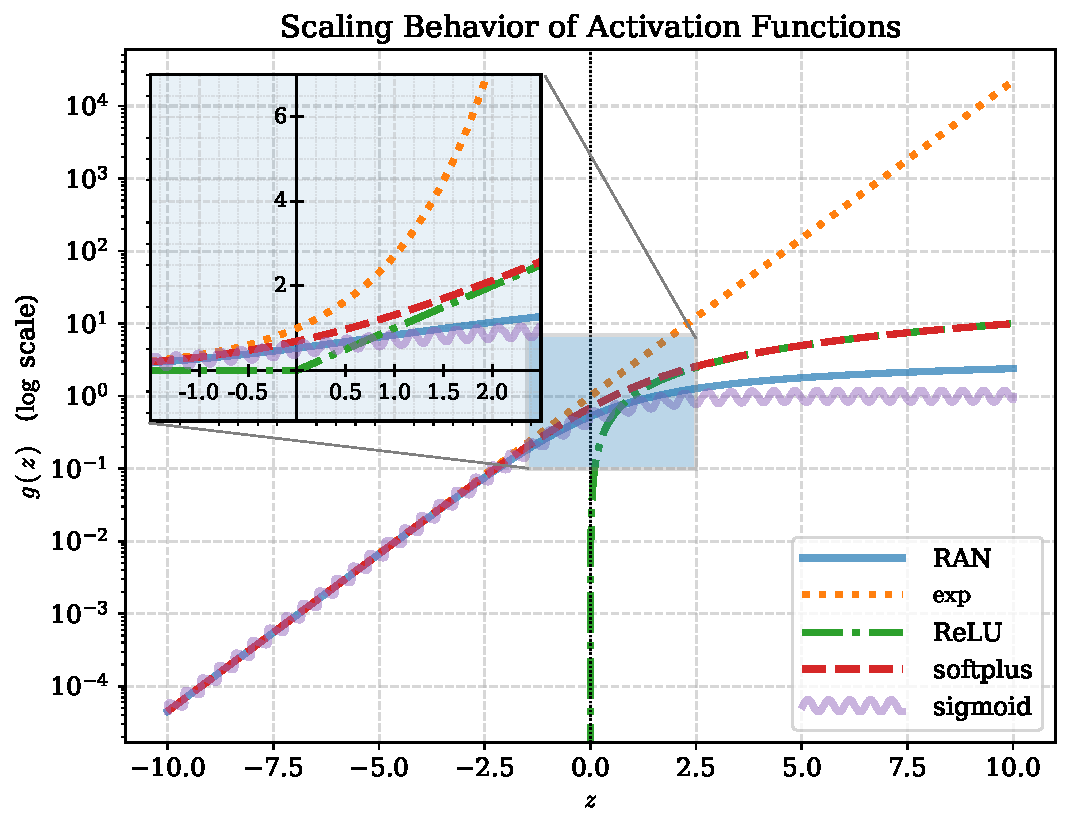
\includegraphics[width=\linewidth]{figures/chapter-06/activations.pdf}
\caption[Comparison of activation functions for neural network weight parametrisation]{Comparison of activation functions considered for parametrising the generator weights $g(z)$. The main plot shows five functions on a logarithmic scale: the custom RAN activation $\log(1 + \text{softplus})$ (blue solid), exponential (orange dots), ReLU (green dash--dot), softplus (red dashed), and sigmoid (violet waved). The gray shaded region indicates the interval $[-2, 2]$, which is shown in detail in the inset with linear scaling. The exponential function exhibits rapid growth for moderately large inputs, while the sigmoid saturates at 1, preventing large weights when needed. ReLU exhibits linear growth, but returns zero gradients for negative inputs. Softplus also exhibits linear growth, but is a smooth function with nonzero gradients for all inputs.
%
The RAN activation balances these extremes, preserving smoothness, positivity, and positive gradients, while transitioning from exponential--like behaviour near zero to logarithmic growth for large $z$, providing numerical stability without imposing hard bounds.}
            \end{figure}
            This adjusted activation guarantees that
            \begin{enumerate}
                \item $g(z) > 0$ for any input, by construction of softplus and log,
                \item \(g(z)\) can still produce arbitrarily large values in principle. This activation function as no finite upper bound, unlike a sigmoid which saturates.%
                This ensures that RAN does not limit the solution space unduly, 
                \item Extremely large weights are disfavored because pushing $f_\theta(z)$ to $\gg 0$ yields only diminishing returns in $g(z)$.
            \end{enumerate}
            
            In practice, this means the network would have to invest a lot of capacity to achieve a huge weight on a single event, which is only worthwhile if doing so reduces the Wasserstein distance significantly.
            %
            Typically, it will be more effective to increase weights more evenly on a group of events covering a region of phase space than to make one weight enormous.
            %
            This activation function thus serves as an internal regulariser, curbing the tendency of the solution to form spikes or outlier weights.
            %
           Since this is a soft constraint, large weights are not forbidden, but the system must pay a price to realise them, much like a physical prior that discourages sharp discontinuities in the solution unless the data demand them.
            %
            The use of this modified activation proves to be crucial for achieving stable training in RAN; with the standard exponential, one observes frequent instances of a single event’s weight blowing up and derailing the fit, whereas the log--softplus activation yields more balanced weight distributions.
            %
        \subsection{Regularising with MC Prior}
            Finally, it is worth noting an intrinsic form of regularisation in RAN that comes ``for free'': by construction, the unfolded result is expressed as a reweighted version of the initial Generation sample.
            %
            This means the unfolded distribution cannot introduce structures that were not present (even in latent form) in the MC.
            %
            In effect, the MC provides a prior support and shape for the solution.
            %
            If the true underlying distribution has features outside the MC’s support, RAN, like any reweighting method, cannot recover them.
            %
            But conversely, it will not produce spurious artifacts that violate known physics encoded in the simulation.
            %
            This is similar in spirit to a Bayesian prior or a template fit: one starts with a template (the Generation) and only deform it as necessary to fit the data.
            %
            The closer the Generation is to reality, the less adjustment is needed.
            %
            RAN’s design choice of ``tweaking a known density rather than learning a new one from scratch'' is motivated by the desire to leverage this built--in regularisation.
            %
            This allows RAN’s solutions to be smoother and more statistically robust than those from unconstrained generative models, precisely because $g(z)$ operates within the scaffolding of the Monte Carlo sample.
            %
            This comes at the cost of some bias if the Monte Carlo is poor, which no method can escape that without additional external input, but is a conscious regularisation choice favouring stability over unrestricted flexibility.

    In summary, the RAN methodology interweaves modern ML techniques with classical regularisation principles to achieve a stable unfolding.
        %
    The use of the Wasserstein distance (WGAN) provides a gentle, physics--aligned way of comparing distributions that avoids the brittleness of binary classification metrics.
        %
     Imposing Lipschitz continuity on the critic via gradient penalties and spectral normalization keeps the adversarial game well--behaved and prevents the discriminator from overemphasising statistical noise.
    %
    On the generator side, starting from the physical prior (simulation) and limiting the capacity for extreme weights (through initialization and activation choices) anchor the solution close to expected physics and discourage overfitting.
    %
    Together, these innovations allow RAN to unfold full distributions in one shot, non--iteratively, without the severe instabilities that one might fear from an unconstrained GAN approach.
    %
    In effect, RAN attains a balance.
    %
    It is flexible enough to accurately fit complex, high--dimensional data, yet sufficiently regularised to suppress unphysical oscillations and variance.
    %
    The result is an unfolding method that achieves competitive or superior performance to iterative methods like \textsc{OmniFold}, while operating in a single training pass and maintaining controlled behaviour even in challenging regimes\footnote{Such as limited detector overlap or low--statistics bins.}.
    %
    The following sections will demonstrate these points quantitatively with examples, but the methodological foundation laid out here is key to understanding why RAN performs as well as it does.
    %
    It marries the strengths of adversarial learning with the hard--earned lessons of regularisation from decades of unfolding research, yielding a novel and powerful approach to this classic problem.
\section{Machine learning implementation.}
\label{sec:ran-ml-implementation}
    \subsection{Neural Network Architecture}
        A Reweighting Adversarial Network (RAN) consists of two components: a \emph{generator} network that assigns event wise weights, and a \emph{critic} network that evaluates the discrepancy between weighted simulation and data.
        %
        RAN implements both as small fully connected, dense, neural networks using the \textsc{TensorFlow~2/Keras} framework for prototyping~\cite{Abadi2016TensorFlow:Learning, chollet2015keras}.
        %
        \footnote{The design is straightforward to reproduce in \textsc{PyTorch} using analogous layers and normalisation techniques.}
        %
        The architecture was kept intentionally simple to ensure stable training and avoid over fitting, with identical layer widths for the generator and critic.

        The generator $g(z;\boldsymbol{\beta})$ takes as input the \emph{particle level} feature vector $z \in \mathbb{R}^{N_T}$ of a generated event, where \(N_T\) is the dimension of the Generation, and the Truth.
        %
        For example, $N_T=1$ for one dimensional toy data or $N_T=6$ for the multi--observable jet dataset described below.
        
        The generator outputs a scalar weight $w=g(z)$ that reweights that event in order to correct the Simulation towards Data.
        %
        The generator is a feed--forward multilayer perceptron with three hidden layers of 50 nodes each.
        %
        Each hidden layer uses a Leaky Rectified Linear Unit (Leaky ReLU) activation~\cite{Maas2013RectifierModels}, with parameter \(\alpha = 0.3.\)
        \[
            \textbf{LeakyReLU} (z;\,\alpha) = \max(z, 0) + \alpha\,\min(0, z).
        \]
        
        Batch normalisation and a dropout of \(20\%\) is applied after each dense layer to promote stable training and reduce overfitting.
        %
        The final layer of the generator is a single linear neuron (no activation) producing a raw scalar $t$.
        %
        This output is then transformed to a positive weight.
        %
        Instead of a direct exponential mapping the stabilised transformation,
        \[ 
            w \;=\; \log\Big(1 + \text{softplus}(t)\Big)\,.
        \]
        is applied to \(t\).
         Finally, the set of weights ${w_i}$ in each mini--batch is normalized so that their average is unity.
         %
         This batch level normalisation means the total weight of the simulated sample remains consistent, preserving overall event counts, by approximating the ``partition function''.
         %
         The generator network thus defines a differentiable reweighting function $g(z)$ that can smoothly adjust the contribution of each simulated event during training.

        The critic $d(x;\,\boldsymbol{\theta})$ is a discriminator--like network that takes as input the detector level feature vector $x \in \mathbb{R}^{N_D}$ of an event and outputs a real valued score.
        %
        This network is tasked with distinguishing the weighted Simulation from the Data in the detector space, and its output is used as an approximate distance measure between the two distributions.
        %
        Like the generator, the critic is implemented as a fully connected network with three hidden layers of 50 nodes each, using Leaky ReLU activations and interleaved batch normalisation and \(20\%\) dropout.
        %
        The output layer is a single linear node producing the critic score $d(x)$.
        
        To satisfy the requirements of the Wasserstein GAN framework, the critic must be a \(1-\)Lipschitz function.
        %
        As discussed, spectral normalization scales the layer weights such that their largest singular value is 1, effectively controlling the Lipschitz constant of $d$ without the need for weight clipping.
        %
        This technique, combined with dropout, greatly improved training stability by preventing the critic from becoming overly sensitive to outlier events.
        %
        Additionally, a mild output clipping is applied to the critic scores, capping $d(x)$ within a reasonable range to eliminate spurious large values that could arise from statistical fluctuations, which in this context would correspond to unphysical negative probabilities or overly large separation scores~\cite{dai_rethinking_2022, arjovsky_wasserstein_2017}.
        %
        A schematic of the RAN architecture is shown in \cref{fig:model-arch}.
        %
        \begin{figure}
    \begin{tikzpicture}[font=\sffamily, >=stealth, node distance=1cm]

% Big dashed box for the Generator
\node[draw, dashed, thick, inner sep=10pt, minimum width=6cm, minimum height=10cm, 
      label={[above left, anchor=west, yshift=-0.5cm, xshift=2.25cm]{\Huge \textbf{$g$}}}] (genBox) {};

% Input arrow into the generator box
\node[above=of genBox.north, yshift=-0.5cm] (genInput) {\large\textbf{Generation} ($z$)};


% Inside the Generator: the repeated block.
% Place the first block in the top-left of the dashed box.
\node[draw, rectangle, rounded corners, fill=green!20, minimum width=2.5cm, minimum height=1cm] 
  (dense) at ([xshift=0.cm,yshift=-1cm]genBox.north) {Dense};
\draw[->, thick] (genInput) -- (dense);
\node[draw, rectangle, rounded corners, fill=green!25, minimum width=2.5cm, minimum height=1cm, below=1cm of dense] 
  (lrelu) {LeakyReLU};

\node[draw, rectangle, rounded corners, fill=green!30, minimum width=2.5cm, minimum height=1cm, below=1cm of lrelu] 
  (bnorm) {BatchNorm};

\node[draw, rectangle, rounded corners, fill=green!30, minimum width=2.5cm, minimum height=1cm, below=1cm of bnorm] 
  (drop) {Dropout(0.2)};

% Connect the blocks in sequence with arrows.
\draw[->, thick] (dense) -- (lrelu);
\draw[->, thick] (lrelu) -- (bnorm);
\draw[->, thick] (bnorm) -- (drop);

% A looping arrow indicating that the Dense -> LeakyReLU -> LayerNorm -> Dropout block is repeated 15 times.
\draw[->, thick, bend left=45] (drop.west) to (dense.west);

% Final block: output layer (outside the loop)
\node[draw, rectangle, rounded corners, fill=green!40, minimum width=2.5cm, minimum height=1cm, below=1cm of drop] 
  (final){exp};

% Connect the looped block to the final block.
\draw[->, thick] (drop) -- (final);

% Output arrow from the generator box.
\node[below=of genBox.south, yshift=0.5cm] (genOutput) {\large\textbf{Event weights} $g(z)$};
\draw[->, thick] (final) -- (genOutput);

\node[draw, dashed, thick, inner sep=10pt, minimum width=6cm, minimum height=10cm, 
      label={[above left, anchor=west, yshift=-0.5cm, xshift=-2.75cm]{\Huge \textbf{$d$}}}] (critBox) [right=3cm of genBox] {};



% Input arrow into the Critic box
\node[above=of critBox.north, yshift=-0.5cm] (critInput) {\large\textbf{Simulation $\vb*{\cup}$ Data} $(x)$};

\coordinate (A) at ($(genOutput.east) + (-0.4,11.76)$);
\draw[-{Latex[length=2mm,width=2mm]}, double, thick, OliveGreen, in=190]
  ($(genOutput.north east)+(-0.4, -0.2)$) -- (A) -- (critInput.west)
  node[midway, below, sloped] {\large \textbf{Induced weights}};
% Inside the Critic: the repeated block (4 times).
\node[draw, rectangle, rounded corners, fill=blue!50, minimum width=2.5cm, minimum height=2cm, 
       label={[yshift=-0.8cm]above:{Spectral Norm}}] 
       (specBox) at ([xshift=0cm,yshift=-1.5cm]critBox.north) {};

\node[draw, rectangle, rounded corners, fill=blue!10, minimum width=2cm, minimum height=1cm] 
       (dense) at ([yshift=-0.3cm]specBox.center) {Dense};
  \draw[->, thick] (critInput) -- (specBox);
  
\node[draw, rectangle, rounded corners, fill=blue!20, minimum width=2.5cm, minimum height=1cm, below=0.5cm of specBox] 
  (sleaky) {LeakyReLU};

\node[draw, rectangle, rounded corners, fill=blue!30, minimum width=2.5cm, minimum height=1cm, below=0.5cm of sleaky] 
  (sdrop) {Dropout};

\node[draw, rectangle, rounded corners, fill=blue!40, minimum width=2.5cm, minimum height=1cm, below=0.5cm of sdrop] 
  (snorm) {LayerNorm};

% Connect these blocks.
\draw[->, thick] (specBox) -- (sleaky);
\draw[->, thick] (sleaky) -- (sdrop);
\draw[->, thick] (sdrop) -- (snorm);

% Looping arrow for the critic repeated block (4 times).
\draw[->, thick, bend right=45] (snorm.east) to (specBox.east);

% Final block for the Critic: output layer.
\node[draw, rectangle, rounded corners, fill=blue!50, minimum width=2.5cm, minimum height=2cm, 
       label={[yshift=-0.8cm]above:{Spectral Norm}}] 
       (sfinal) [below=0.5cm of snorm] {};
       
\node[draw, rectangle, rounded corners, fill=blue!10, minimum width=2cm, minimum height=1cm] 
       (slinear) at ([yshift=-0.3cm]sfinal.center) {Linear};

\draw[->, thick] (snorm) -- (sfinal);

% Output arrow from the Critic box.
\node[below=of critBox.south, yshift=0.5cm] (critOutput) {\large\textbf{Critic Score} $d(x)$};
\draw[->, thick] (sfinal) -- (critOutput);

\node[draw, ellipse, thick, fill=red!10, minimum width=3cm, minimum height=2cm] (lossNode) at ($(genBox)!0.5!(critBox) + (0,-3cm)$) {\large\textbf{Wasserstein Loss}};

\draw[-{Latex[length=2mm, width=2mm]}, double, RoyalBlue, bend left=45, thick](critOutput.west) to (lossNode);

\node (junction) at ($(lossNode.north) + (0,1.5cm)$) {};

% Draw the common arrow from the loss node to the junction,
% and label that common segment.
\draw[-, double, red, thick]
  (lossNode.north) -- (junction.north)
  node[near end, above, sloped]{\large\textbf{Gradient}}node[near end, below, sloped]{\large\textbf{Update}};

% From the junction, branch off to the two big boxes.
\draw[-{Latex[length=2mm,width=2mm]}, double, red, thick] (junction.north) to[out=90, in=-60]  ($(genBox.north east)+(-0.5,-0.9)$)
  node[very near start, above, sloped]{};
\draw[-{Latex[length=2mm,width=2mm]}, double, red, thick] (junction.north) to[out=90, in=-120] ($(critBox.north west)+(.5,-0.9)$)
  node[midway, above, sloped]{\quad};



\end{tikzpicture}
    \caption[RAN architecture with generator and critic networks]{Architecture of the Reweighting Adversarial Network (RAN). 
    \textbf{Left:} The generator network processes particle level features through three hidden layers (50 nodes each) with LeakyReLU activation, batch normalization, and 20\% dropout. The output layer produces non negative event weights using the log--softplus activation.
    \textbf{Right:} The critic network evaluates detector level features through spectrally normalised dense layers with LeakyReLU activation, layer normalisation, and dropout, outputting a scalar critic score.
    %
    The networks are trained adversarially using a Wasserstein loss with gradient penalty, where the critic learns to distinguish weighted Simulation from Data while the generator learns to reweight Generation such that the induced weights on Simulation minimise this distinction.}
    \label{fig:model-arch}
\end{figure}

        The balanced capacity of the generator and critic, each with $\mathcal{O}(10^4)$ trainable parameters, was found sufficient to learn the required reweighting functions without overfitting, given the complexity of the tasks considered.

    \subsection{Adversarial training procedure.}
        Training a RAN involves a minimax game between the generator and critic, similar in spirit to a Generative Adversarial Network (GAN).
        %
        However, unlike a standard GAN that generates new events, RAN's generator only reweights existing events.
        %
        RAN adopts the Wasserstein GAN (WGAN) approach for improved stability.
        %
        The critic’s objective is to maximise the statistical distance, in the Wasserstein--1 sense, between the weighted simulation and the true data distributions at the detector level, while the generator’s objective is to produce weights for Generation such that the induced weights on Simulation minimise this distance.
        %
        Formally, let $p(x)$ be the true data distribution in detector space and $q(z, x)$ be the joint distribution of generation and simulation.
        %
        At each training step, the critic $d$ is trained to minimize the loss function
        \[
            L_d = -\mathbb{E}_{x\sim p}[\,d(x)\,]\;+\;\mathbb{E}_{(z, x)\sim q}\big[\,g(z)\,d(x)\,\big]\,,
            \label{eq:wgan_loss}
        \]
        where $(z, x)$ denotes a corresponding Generation and Simulation event pair.
        %
        $-L_d$ is an empirical estimate of the Wasserstein\(-1\) distance between Data and reweighted Simulation.
        %
        The generator, on the other hand, is trained to maximise this same quantity (equivalently, to minimize the negative critic loss $-L_d$), thereby pushing the weighted Simulation to resemble the Data.
        
        Unlike the binary cross--entropy loss in a traditional GAN, the Wasserstein formulation provides a smooth, continuous loss landscape even when the two distributions do not overlap perfectly.
        %
        This is helpful for unfolding problems because even if detector effects cause $p(x)$ and the original $q(x)$ to have non-overlapping support in $x$, the WGAN critic can still provide informative gradients to the generator.
        %
        This choice eliminates the severe mode collapse or large weight oscillations that occur when using the BCE loss in extant classifier based methods.
        %
        The WGAN’s stronger theoretical guarantees, combined with the property that RAN only classifies at detector level, and only reweights at particle level, ensure the training remains well behaved even with minimal overlap~\cite{gulrajani_improved_2017}
        
        To further enforce the \(1-\)Lipschitz condition required by the Wasserstein theory, one can include a gradient penalty term in the critic’s loss.
        %
        This penalty,
        \[
            L_{GP} = \lambda\,\mathbb{E}_{\hat{x}}\qty[(\norm{\nabla_{\hat{x}}d(\hat{x})}_2 - 1)^2],
        \]
        is computed on randomly sampled points $\hat{x}$ uniformly interpolated between Data and reweighted Simulation.
        %
        $\lambda$ usually set between five and ten.
        %
        The gradient penalty, together with spectral normalisation, acts as a robust regulariser against critic over--training.

        Training proceeds by alternating between critic and generator updates in each iteration, following the typical WGAN--GP strategy.
        %
        The studies presented below used an update ratio of 3:2 for the critic:generator, meaning the critic is updated slightly more frequently to keep it near optimality as the generator evolves.
        %
        Pseudocode for one training cycle is outlined in Algorithm~\ref{alg:wgan-gp}.

        \begin{algorithm}
            \caption{WGAN GP Training Step}
            \label{alg:wgan-gp}
            \KwIn{
              Data distribution $p(x)$, 
              Generation, Simulation pairs \(q(z, x)\),
              critic $d_{\theta}$, 
              generator weights $g(z;\beta)$,\\
              gradient penalty weight $\lambda$, 
              critic steps $n_c$, 
              generator steps $n_g$, 
              batch size $B$
            }
            \KwOut{Trained parameters $\theta$ and $\beta$}
        \For{iteration $=1,2,\dots$}{
          \tcp{Critic updates}
          \For{\(i\) in \(1\) \KwTo $n_c$}{
            Sample $\{x_i^{\text data}\}_{i=1}^B\sim p(x)$\;
            Sample $\{(z_j, x_j\}_{j=1}^B\sim q(z, x)$\;
            Compute $w_j = g(z_j;\beta)$\;
            Compute
            \[
              L_d
              = \frac1B\sum_{i=1}^B d_{\theta}(x_i^{\text data})
                -\frac1B\sum_{j=1}^B w_j\,d_{\theta}\bigl(x^{\text sim}_j\bigr)
                +\lambda\,L_{\text GP}(\theta)\,;
            \]
            $\theta \;\leftarrow\;\theta + \eta_d\,\nabla_{\theta}L_d$\;    
          }
        
          \tcp{Generator updates}
          \For{\(j\) in \(1\) \KwTo $n_g$}{
            Sample fresh $\{x_i^{\text{data}}\}_{i=1}^B\sim p(x)$\;
            Sample $\{(z_j, x_j\}_{j=1}^B\sim q(z, x)$\;
            Compute $w_j = g(z_j;\beta)$\;
            Compute
            \[
              L_g 
              = -\frac1B\sum_{j=1}^B w_j\,d_{\theta}\bigl(x_j^{\text{ sim}})\bigr)
                + \frac1B\sum_{i=1}^B d_{\theta}(x_i^{\text{data}})\,;
            \]
            $\beta \;\leftarrow\;\beta - \eta_g\,\nabla_{\beta}L_g$\;
          }
        }
        \end{algorithm}
        These steps constitute one training iteration, and they are repeated until convergence criteria are met.
        %
        Both networks are optimised using the RMSProp optimiser, which was found to outperform \textsc{Adam} in the WGAN setting, ,consistent with previous studies~\cite{henderson_where_2018}
        %
        The learning rate for both generator and critic are set in the range $\eta \sim 1\times10^{-4}$ to $5\times10^{-4}$, with the exact value tuned per dataset.
        %
        A need for explicit learning rate decay schedules beyond those automatically implemented by \textsc{Keras}, was not observed as training typically converged to a stable solution before any signs of stalling.
        %
        A mini--batch size of $B=256$ was used for all experiments, providing a good balance between gradient estimate stability and computational efficiency.
        
        The studies presented in this chapter do not involve an exhaustive hyperparameter search; instead, they rely on standard GAN/WGAN settings from the literature and minor tuning.
        %
        In practice, the performance of RAN is found to be robust against moderate changes in these settings: for instance, altering the learning rate by a factor of two or using 40 or 60 nodes per layer, instead of 50, had no significant impact on the final unfolded distributions.
        %
        This insensitivity suggests that the RAN method does not require fine--tuned hyperparameters to achieve reliable results, an important consideration for reproducibility.
    
        Throughout training, key loss terms  should be continuously monitored to ensure the optimisation remains stable.
        %
        In particular, one should track the Wasserstein critic loss $L_d$ and the gradient penalty magnitude.
        %
        A sharp increase in the gradient penalty or a sudden large oscillation in $L_d$ can indicate that the critic is violating the Lipschitz constraint or that the generator is producing pathological weights, a potential onset of mode collapse.
        %
        If such behaviour is observed, one can intervene by pausing training and lowering the learning rate or increasing regularisation before resuming from the last stable checkpoint.
        
        In the experiments presented, the use of spectral normalisation and gradient penalty together largely prevented such divergences.
        %
        Here, it is important to re-emphasise that RAN’s one shot training, as opposed to an iterative approach, simplifies the overall optimisation schedule.
        %
        Once the adversarial equilibrium is reached, one immediately obtains the final reweighting function without needing multiple retraining cycles.
    
    \subsection{Datasets and preprocessing.}
        The aforementioned architecture and training procedure was applied to two representative unfolding scenarios: a controlled \(1-\)dimensional Gaussian example and a realistic high--dimensional jet physics example.
        %
        These two cases allow one to validate the RAN implementation on both simple and complex distributions.

        \subsubsection{Gaussian example.}
            The first dataset is a synthetic scenario with known analytical truth, designed to illustrate RAN’s behavior under varying degrees of detector smearing.
            %
            Generate two sets of events from normal distributions at the particle level, a ``Truth'' distribution $Z_{\text{T}} \sim \mathcal{N}(\mu_{\text{Truth}},\,1)$ and a ``Generation'' distribution $Z_{\text{G}} \sim \mathcal{N}(\mu_{\text{Gen.}},\,1)$, with means $\mu_{\text{Truth}}=0$ and $\mu_{\text{Gen.}}=-1$.
            %
            Sample \(\num{d4}\) events from the Truth distribution and \(\num{d5}\) events from the generation distribution.
            
            To emulate detector effects, each particle-level value $z$ is transformed by a simple deterministic response: $x = S \cdot z$, where $S$ is a scalar ``smearing'' factor which is constant for any given individual unfolding experiment.
            %
            For example, when $S=1,$ the Data equals the Truth with no smearing, while $S>1$ stretches the distribution, reducing the overlap between the Data ($X_D = S\cdot Z_{\text{T}}$) and Simulation ($X_S = S\cdot Z_{\text{G}}$).
            %
            Data is unfolded over a range of \(S\) values representing increasingly degraded detector responses.
            
            Since this is a one dimensional setup, \(N_T = N_D = 1\) i.e, each event is described by a single number.
            %
            Apart from the deterministic scaling, no additional noise or inefficiency is introduced, so the challenge lies purely in the shift of distributions and, more importantly the lack of detector level support overlap as $S$ grows large.
            %
            No additional preprocessing of the input features is necessary since they are already standardised aside from mean shifts and bounded.
            
            During training, at each iteration draw a random batch of $B=256$ values from the $\num{d4}$ available smeared Data points and another batch of 256 from the $\num{d5}$ smeared Simulation points.
            %
            Because the Simulation sample is larger, cycle through it randomly shuffled such that multiple data epochs correspond to one pass through the simulation.
            %
            It is beneficial to shuffle and reshuffle both samples frequently during training to avoid any periodic artifacts given the fixed deterministic smearing.
            
            The generator is tasked with learning event weights $g(z)$ that correct the Generation distribution centred at $-1$ to match the true distribution centred at 0, using only classification information from the $X$ domain where in extreme cases the distributions barely overlap.
            
            This toy example is especially useful for validating the implementation because the optimal reweighting function is known.
            %
            In the limit of infinite statistics, the optimal weight would be proportional to the ratio of Truth to Generation densities at $z$, which in this case is $\exp[-(z-\mu_{\text{Truth}})^2/2 + (z-\mu_{\text{Gen.}})^2/2]$, a Gaussian weight.
            %
            It also allows one to verify that RAN’s adversarial training indeed converges to the correct solution, by comparing the unfolded distribution to the analytic expectation.

        \subsubsection{Jet substructure dataset}
            The second dataset studied is a realistic example taken from high energy physics, involving the unfolding of jet substructure observables.
            %
            For this experiment, follow the setup of the \textsc{OmniFold} study described in~\cite{andreassen_omnifold_2020} to enable direct comparisons.
            %
            Proton--proton collision events at $\sqrt{s}=14$~TeV are generated using two different Monte Carlo simulators, \textsc{Pythia}8.243~\cite{Sjostrand:2014zea, Sjostrand:2007gs} with Tune 26~\cite{TheATLAScollaboration:2014rfk} provides the initial Generation sample, and \textsc{Herwig}~7.1.5~\cite{Bellm2017HerwigNote, Bahr:2008pv} is used to generate an independent sample treated as the Truth distribution.
            %
            Each event in both samples contains a high-$p_T$ $Z$ boson with $p_T^Z > 200$~GeV decaying leptonically, produced back to back with a hadronic jet.
            %
            The presence of a $Z$ boson trigger ensures a well defined event sample and reduces acceptance differences.
            %
            The final state particles in each event are passed through a fast detector simulation using \textsc{Delphes}~3.4.2~\cite{DeFavereau2014DELPHESExperiment} with a CMS detector configuration including particle flow reconstruction~\cite{Mertens:2015kba, CMS:2017yfk}.
            %
            Jets are then reconstructed in both the particle--level and detector--level event records using the anti$-k_T$ clustering algorithm~\cite{Cacciari:2008gp} with a radius parameter, $R=0.4$, as implemented in \textsc{FastJet}3.3.2~\cite{Cacciari2012FastJetManual}
            
            This dataset focuses on the hardest jet in each event, the jet that balances the $Z$ boson’s recoil, to define its observables.
            %
            For each jet, consider six different substructure observables that characterise its internal pattern of particles.
            %
            These include classic measures like the jet mass $m$ and jet breadth or width $w$, as well as more specialized variables such as the \(N-\)subjettiness ratio $\tau_{21}$, the groomed momentum fraction $z_g$ from the Soft Drop algorithm, and a logarithmic version of the dimensionless jet mass $\ln\rho$.
            %
            Precise definitions of these observables follow those in \cite{andreassen_omnifold_2020}.
            %
            In total, each jet is described by a feature vector of $N_T = N_D = 6$ numbers (since the same set of observables is defined at particle level and, after \textsc{Delphes} simulation, at detector level).
            %
            These six features form the input to the RAN networks.
            
            It is helpful to whiten (z--score) these inputs to minimise finite precision and overflow errors.
            %
            Prepared the data such that the particle level Truth sample from textsc{Herwig} contains on the order of $\num{d6}$ jets, and the  particle level Generation sample from \textsc{Pythia}, a similar order of magnitude.
            %
            The detector level representations for each sample are obtained via the same \textsc{Delphes} procedure, yielding paired $(z, x)$ examples for \textsc{Pythia} and independent $x$ examples for \textsc{Herwig}.
            
            During training, treat the \textsc{Delphes+Herwig} jets as the Data distribution $p(x)$ and the \textsc{Delphes+Pythia} jets as the initial Simulation, $q(x)$.
            %
            At each iteration, mini-batches of $B=256$ jets are drawn from each distribution.
            %
            Given the relatively large size of the samples, one need not worry about cycling through the data too many times and can simply train for a fixed number of iterations determined by early stopping.
            %
            Ensure that each jet in the training sample is used many times over the course of training, which is important for the generator to refine the weights on all regions of phase space..
            %
            Once training is complete, the learned weights $w = g(z)$ can be applied directly to the Generation events to produce an unfolded distribution for each observable, which we can then compare to the Truth, i.e. \textsc{Herwig} particle level distribution.
            
            It is important to emphasise that in this experiment the ``data'' is fully simulated, \textsc{Herwig+Delphes} rather than experimental observations or measurements.
            %
            This is a common practice in validation studies, allowing us to quantitatively evaluate the accuracy of the unfolding by comparing to known truth.
            %
            However, as is the case with any proposed method, the gold standard of its quality will be demonstrated through future work applying it to real experimental data.

    \subsection{Training, monitoring and validation.}
        To ensure reliable performance and prevent overtraining, one should employ a rigorous monitoring and validation regimen during RAN training.
        %
        First, one should partitioned each dataset into a training set used to update network parameters, a smaller validation set, used for performance monitoring during the training, and a testing set.
        %
        The ratios used were training : validation : testing \(= 70:15:15.\)
        %
        The validation data is not seen by the networks during gradient updates, but one computes the same losses on it to check how well the model generalizes.
        %
        Specifically, after every fixed number of training iterations, one evaluates the critic loss $L_d$ on the validation batch and tracks its evolution.
        %
        If one observes the validation loss starting to increase while the training loss continues to decrease, this is a clear sign of overfitting i.e. the critic is learning spurious differences that do not generalise, or the generator is over adjusting to peculiarities of the training sample.
        %
        In such cases, one should invoke an \emph{early stopping} criterion.
        %
        In the implementation described, early stopping is triggered if the validation Wasserstein distance, approximated by $-L_f$ on the validation set, has not improved for 10 consecutive evaluation intervals.
        %
        Once triggered, one stops training and rolls back to the generator state that had the best validation performance.
        %
        This strategy ensures that one did not overtrain the critic to exploit statistical noise, which would manifest as unstable weights when applied to hitherto unseen validation data.

        In addition to the WGAN loss, one can track several other high level divergence metrics between the reweighted Generation and Truth distributions.
        %
        While these metrics are not used to train the model, since truth is not known in real applications, they are extremely useful to diagnose convergence and compare to alternative methods.
        %
        One such metric is the \textbf{Wasserstein-1 distance} itself between the weighted and true distributions.
        %
        Although the critic provides an estimate of this distance at detector level via the loss, one can also compute it at particle level independently for simpler cases.
        %
        For the 1D Gaussian example, the Wasserstein distance has a closed form which reduces to the difference in means when both distributions are Gaussian with equal width, and for the jet observables one can calculate one dimensional Wasserstein distances for each observable’s distribution individually.
        %
        One can also monitor the Vincze–Le Cam (VLC) divergence, introduced in \cref{subsubsec:distributional-distance-metrics}, between the unfolded reweighted Generation and the Truth.
        Lower values indicate closer agreement between distributions and $\Delta_{VLC}=0$ if and only if $p=q$.
        %
        This metric is particularly sensitive to differences in the tails of distributions and provides complementary check to the Wasserstein distance.
        
        During training, one could periodically apply the current set of weights $g(z)$ to a large sample of simulation events and then evaluate $\Delta_{VLC}$ and the Wasserstein distance between this weighted sample and the truth sample using the known Truth events in validation studies.
        %
        A decreasing trend in both metrics as training progresses signals that RAN is converging towards the correct reweighting.
        
        For instance, in the Gaussian example with moderate smearing, one observes the VLC divergence between the weighted Generation and Truth drop rapidly in the first few dozen epochs and then flatten out at a low value, indicating that the generator had found an effective weighting scheme.
        %
        Similar behaviour is seen in the jet case: the combined six-dimensional weight optimisation gradually improves the agreement in all observables.
        %
        By the end of training, the unfolded distributions for all six jet observables are nearly indistinguishable from the truth, as quantified by final Wasserstein distances on the order of $10^{-2}$ and VLC divergence on the order of $10^{-3}$.\footnote{See~\cite{andreassen_omnifold_2020} for comparable benchmarks involving iterative methods.}
        
        Summary tables \cref{tab:comp_wass, tab:comp_vlc} are included in \cref{sec:ran-results} comparing these divergence metrics for RAN versus other methods; the RAN implementation achieves competitive or superior scores, validating the training procedure described.

        Crucially, the monitoring process also guards against the possibility of divergence or weight blow up.
        %
        If at any point the training appears to destabilise\footnote{E.g., the critic loss oscillates wildly or the weights $\qty{g(z)}$ start to become extremely large for a small subset of events,}, one can intervene by stopping early and/or introducing additional regularization.
        %
        In practice, thanks to the regularisation implemented (spectral norm, gradient penalty, dropout), such pathological behaviour was rare.
        
        One symptom one might encounter in some trials is the appearance of a few very large weights in sparsely populated regions of phase space.
        %
        This is a known issue in unfolding problems.
        %
        When there are regions that have little MC density but non-negligible data density, any reweighting based method will assign large weights to the few simulation events in that region, and RAN is no exception.
        %
        Nonetheless, the spectral normalisation on the critic help limit how fast and how large those weights could grow.
        %
        If needed, one could impose an explicit cap on weights or an additional \(L_p\) norm term in the loss to penalize overly large weights, but this was not found to be necessary for these benchmarks.

    In summary, the ML implementation of RAN described above provees to be robust and reproducible across the different datasets.
    %
    By carefully specifying the architecture with sufficient complexity to learn the needed reweighting, but regularised to avoid overfitting, by using a stable training objective in the Wasserstein divergence with gradient penalty and optimiser, RMSProp, and by employing diligent monitoring and early stopping criteria, one ensures that the training converges reliably to a good solution.
    
    The design choices were informed by both theoretical considerations such as the advantage of WGAN for non-overlapping support and practical experimentation like the choice of 3 critic updates per 2 generator updates for efficiency.
    %
    The resulting RAN model can be straightforwardly re-implemented in common deep learning frameworks and the reported hyperparameters can serve as a baseline for future applications.
    %
    All training scripts and data will be made available open--source to facilitate verification and reuse.

\section{Results}
    \label{sec:ran-results}
    This section evaluates the Reweighting Adversarial Network (RAN) on the two case studies described in the preceding section.
    %
    In each case, RAN’s performance is compared to two baseline methods, the \textsc{OmniFold} algorithm and Iterative Bayesian Unfolding (IBU).
    %
    Quantitative divergence metrics are reported for each method that measure their ability to reproduce the Truth distributions, as well as the methods’ stability under statistical fluctuations.

    \subsection{Gaussian model with smearing.}
        This study represents a targeted unfolding scenario to stress test RAN in a regime of limited detector level overlap.
        %
        As the smearing factor increases above unity, the Data and Simulation become increasingly separated, with less and less overlapping support, even though the underlying particle level distributions remain fixed.
        %
        This controlled setup allows an examination how each unfolding method copes with a progressively worsening mismatch between the Data and Simulation.
        %
        Notably, methods like \textsc{OmniFold} rely reweighting at the detector level, which can fail if the detector--level supports do not overlap well.
        %
        In contrast, RAN performs reweighting at particle level and uses an optimal transport based loss to compare detector level outputs.
        %
        One therefore expects RAN to be more robust in scenarios with poor detector level overlap, provided the particle level distributions still cover each other.

        To quantify performance the Vincze–-Le Cam (VLC) divergence $\Delta_{VLC}$ between the unfolded outcome and the true distribution are used as metrics of accuracy.
        %
        \cref{fig:omnifold-comp} summarizes the unfolding accuracy as a function of the smearing factor, with $\Delta_{\text{VLC}}$ plotted for RAN and \textsc{OmniFold}.

        At minimal smearing, both methods perform excellently, and \textsc{OmniFold} achieves a slightly smaller divergence to truth than RAN.
        %
        For example, at smearing $S = 1, \Delta_{\text{VLC}}$ for \textsc{OmniFold} is $0.057\times10^{-3}$, compared to RAN’s $0.122\times10^{-3}$.
        %
        This confirms that when the detector effects are small and distributions have good support, the problem reduces to a straightforward reweighting and \textsc{OmniFold}’s direct classifier based approach is very effective.
        %
        Indeed, it finds a nearly perfect weighting in this regime.

        However, as the smearing increases and detector level overlap deteriorates, \textsc{OmniFold}’s performance degrades.
        %
        Beyond a smearing factor of about $5$, the \textsc{OmniFold} solution’s divergence from truth grows significantly.
        %
        By the highest smearing values tested, where the Simulation and Data distributions are almost disjoint, \textsc{OmniFold}’s unfolded result significantly deviates from the true distribution, nearly two orders of magnitude worse $\Delta_{VLC}$ compared to the no smearing case.
        
        These observations are consistent with expectations.
        %
        \textsc{OmniFold} tries to reweight at detector level, and when it cannot find common phase space between Data and Simulation, it struggles to assign meaningful weights.
        %
        In stark contrast, RAN maintains a stable performance across the entire range of smearings.
        %
        As shown in \cref{fig:omnifold-comp}, RAN's $\Delta_{\text{VLC}}$ remains approximately constant, with only slight variation within statistical error, as smearing increases.
        %
        Even at the largest smearing factors, RAN's divergence with Truth is essentially the same as it was at zero smearing, indicating that RAN successfully unfolds the distribution despite separation in detector level distributions.
        %
        This behaviour can be attributed to RAN's methodological property of only reweighting at particle level, combined with its use of an optimal transport loss at detector level, which, unlike a classifier, does not require overlapping support to provide a meaningful gradient---the adversarial training can adjust weights to minimize the Wasserstein distance between the smeared Simulation and Data, even if those distributions are partially disjoint.
        %
        The error bars in \cref{fig:omnifold-comp}, representing 1$\sigma$ uncertainties computed by bootstrapping the experiment, confirm the statistical stability of each method.
        %
        RAN’s results are consistent across bootstrap resamples, and while \textsc{OmniFold}’s uncertainty also grows with smearing.
        %
        In summary, this Gaussian study demonstrates that RAN is robust to limited detector level support, recovering the true distribution reliably in a single pass, whereas \textsc{OmniFold} requires sufficient detector level overlap to perform optimally.
        %
        This advantage of RAN becomes valuable in scenarios where detector effects can be large.
\begin{figure}
    \centering
    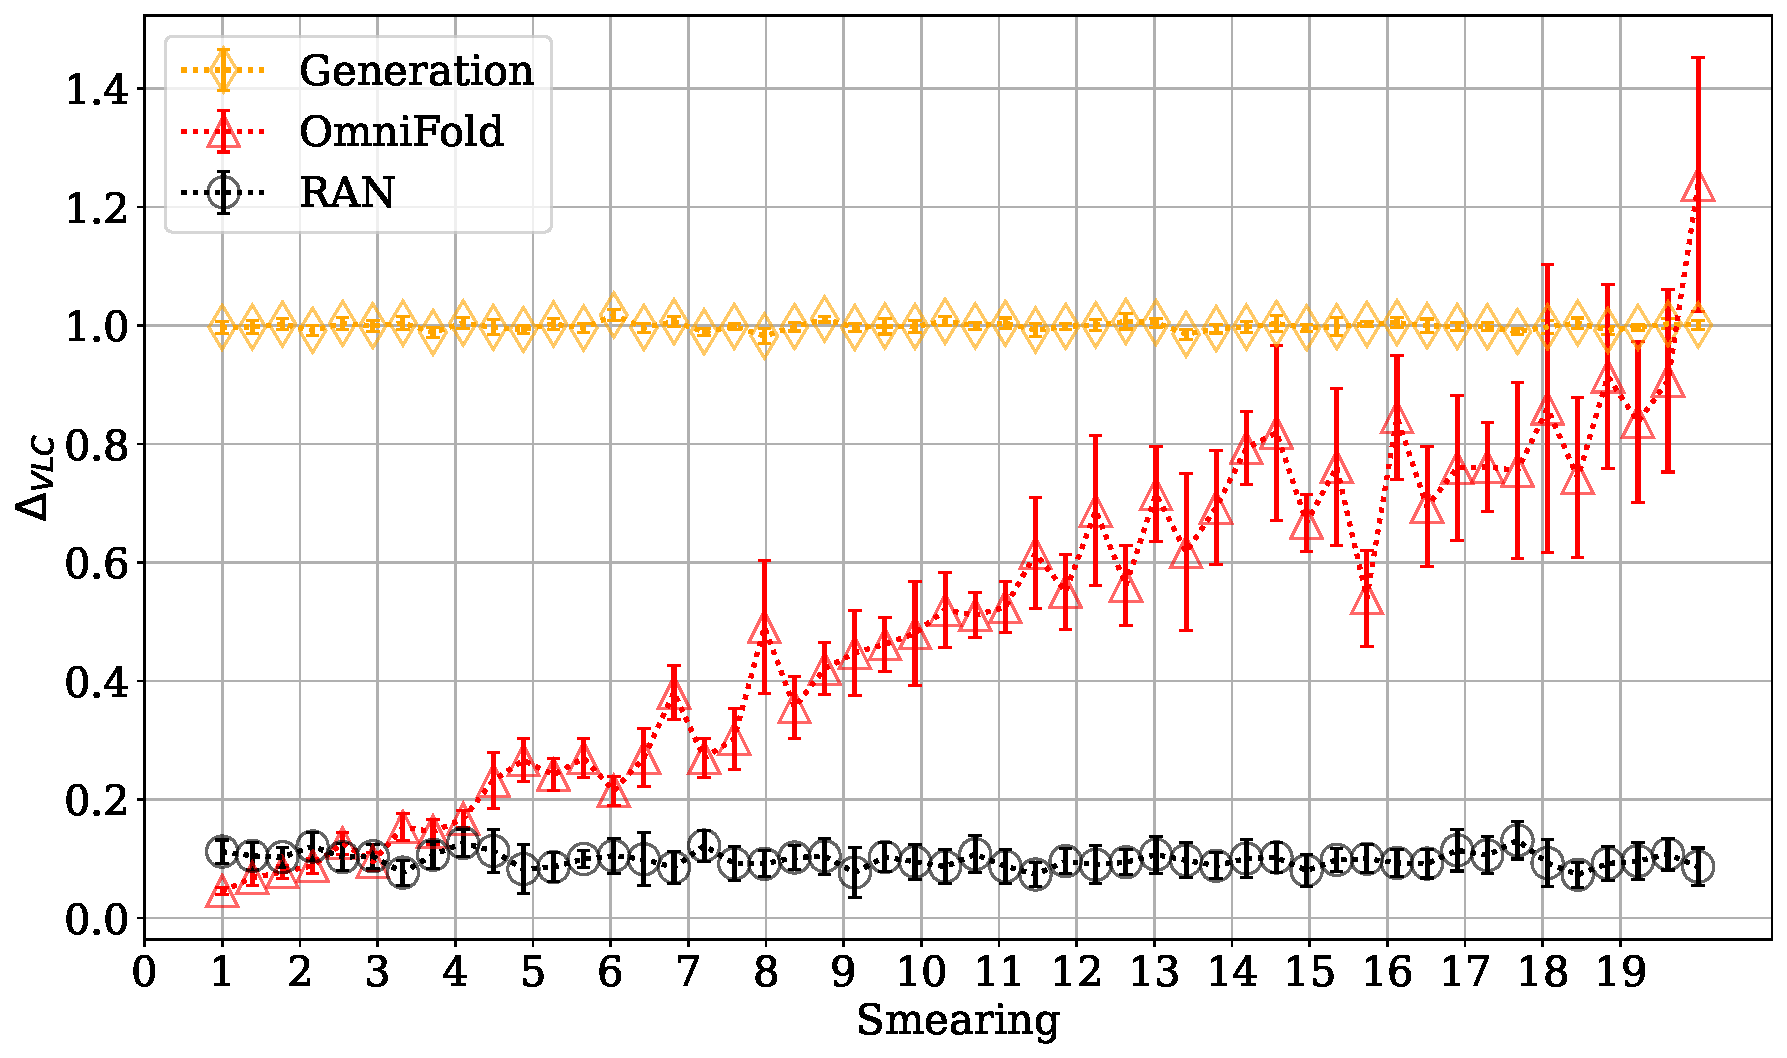
\includegraphics[width=\linewidth]{figures/chapter-06/OF_delta.pdf}
    \caption[Unfolding performance comparison between RAN and OmniFold under varying detector smearing]{Comparison of unfolding performance under increasing detector smearing. 
    The Vincze--Le Cam divergence ($\Delta_{\text{VLC}}$) between unfolded and true distributions is shown as a function of the smearing factor for RAN (black circles) and OmniFold (red triangles). 
    While OmniFold achieves slightly better accuracy at minimal smearing, its performance degrades sharply as smearing increases, reflecting its reliance on detector-level overlap. 
    In contrast, RAN maintains stable performance across all smearing levels, demonstrating robustness to limited detector-level support. 
    The particle-level simulation baseline (yellow diamonds) is shown for reference. 
    Error bars indicate 1$\sigma$ bootstrap confidence intervals.}
    \label{fig:omnifold-comp}
\end{figure}
    \subsection{Jet substructure unfolding results.}
        This study assesses RAN on a realistic high energy physics unfolding task involving correcting jet substructure observables from detector level Data (simulated) to particle level Truth.
        %
        This example serves as a stringent test of RAN’s ability to handle multidimensional, non-Gaussian distributions a range of complex features and long tails.
        %
        The observables chosen span a range of distribution shapes---from broad distributions to sharply peaked ones and those with kinematic cutoffs---providing a comprehensive test-bed.
        %
        RAN is applied to learn a single weighting function $g(z)$ that assigns a single weight to each six dimensional Generation event based on its features to achieve this alignment between Data and reweighted Simulation, as described in \cref{sec:ran-methodology-and-regularisation,sec:ran-ml-implementation}.
        %
        For comparison \textsc{OmniFold} and the classical IBU are also applied to the same task.
        %
        Since IBU is a binned algorithm, one must perform separate one--dimensional IBU unfolds for each observable using a fine histogram binning, to benchmark its performance on each one dimensional projection of the data.

        \subsubsection{Overall performance.}
\begin{figure}
    \centering
    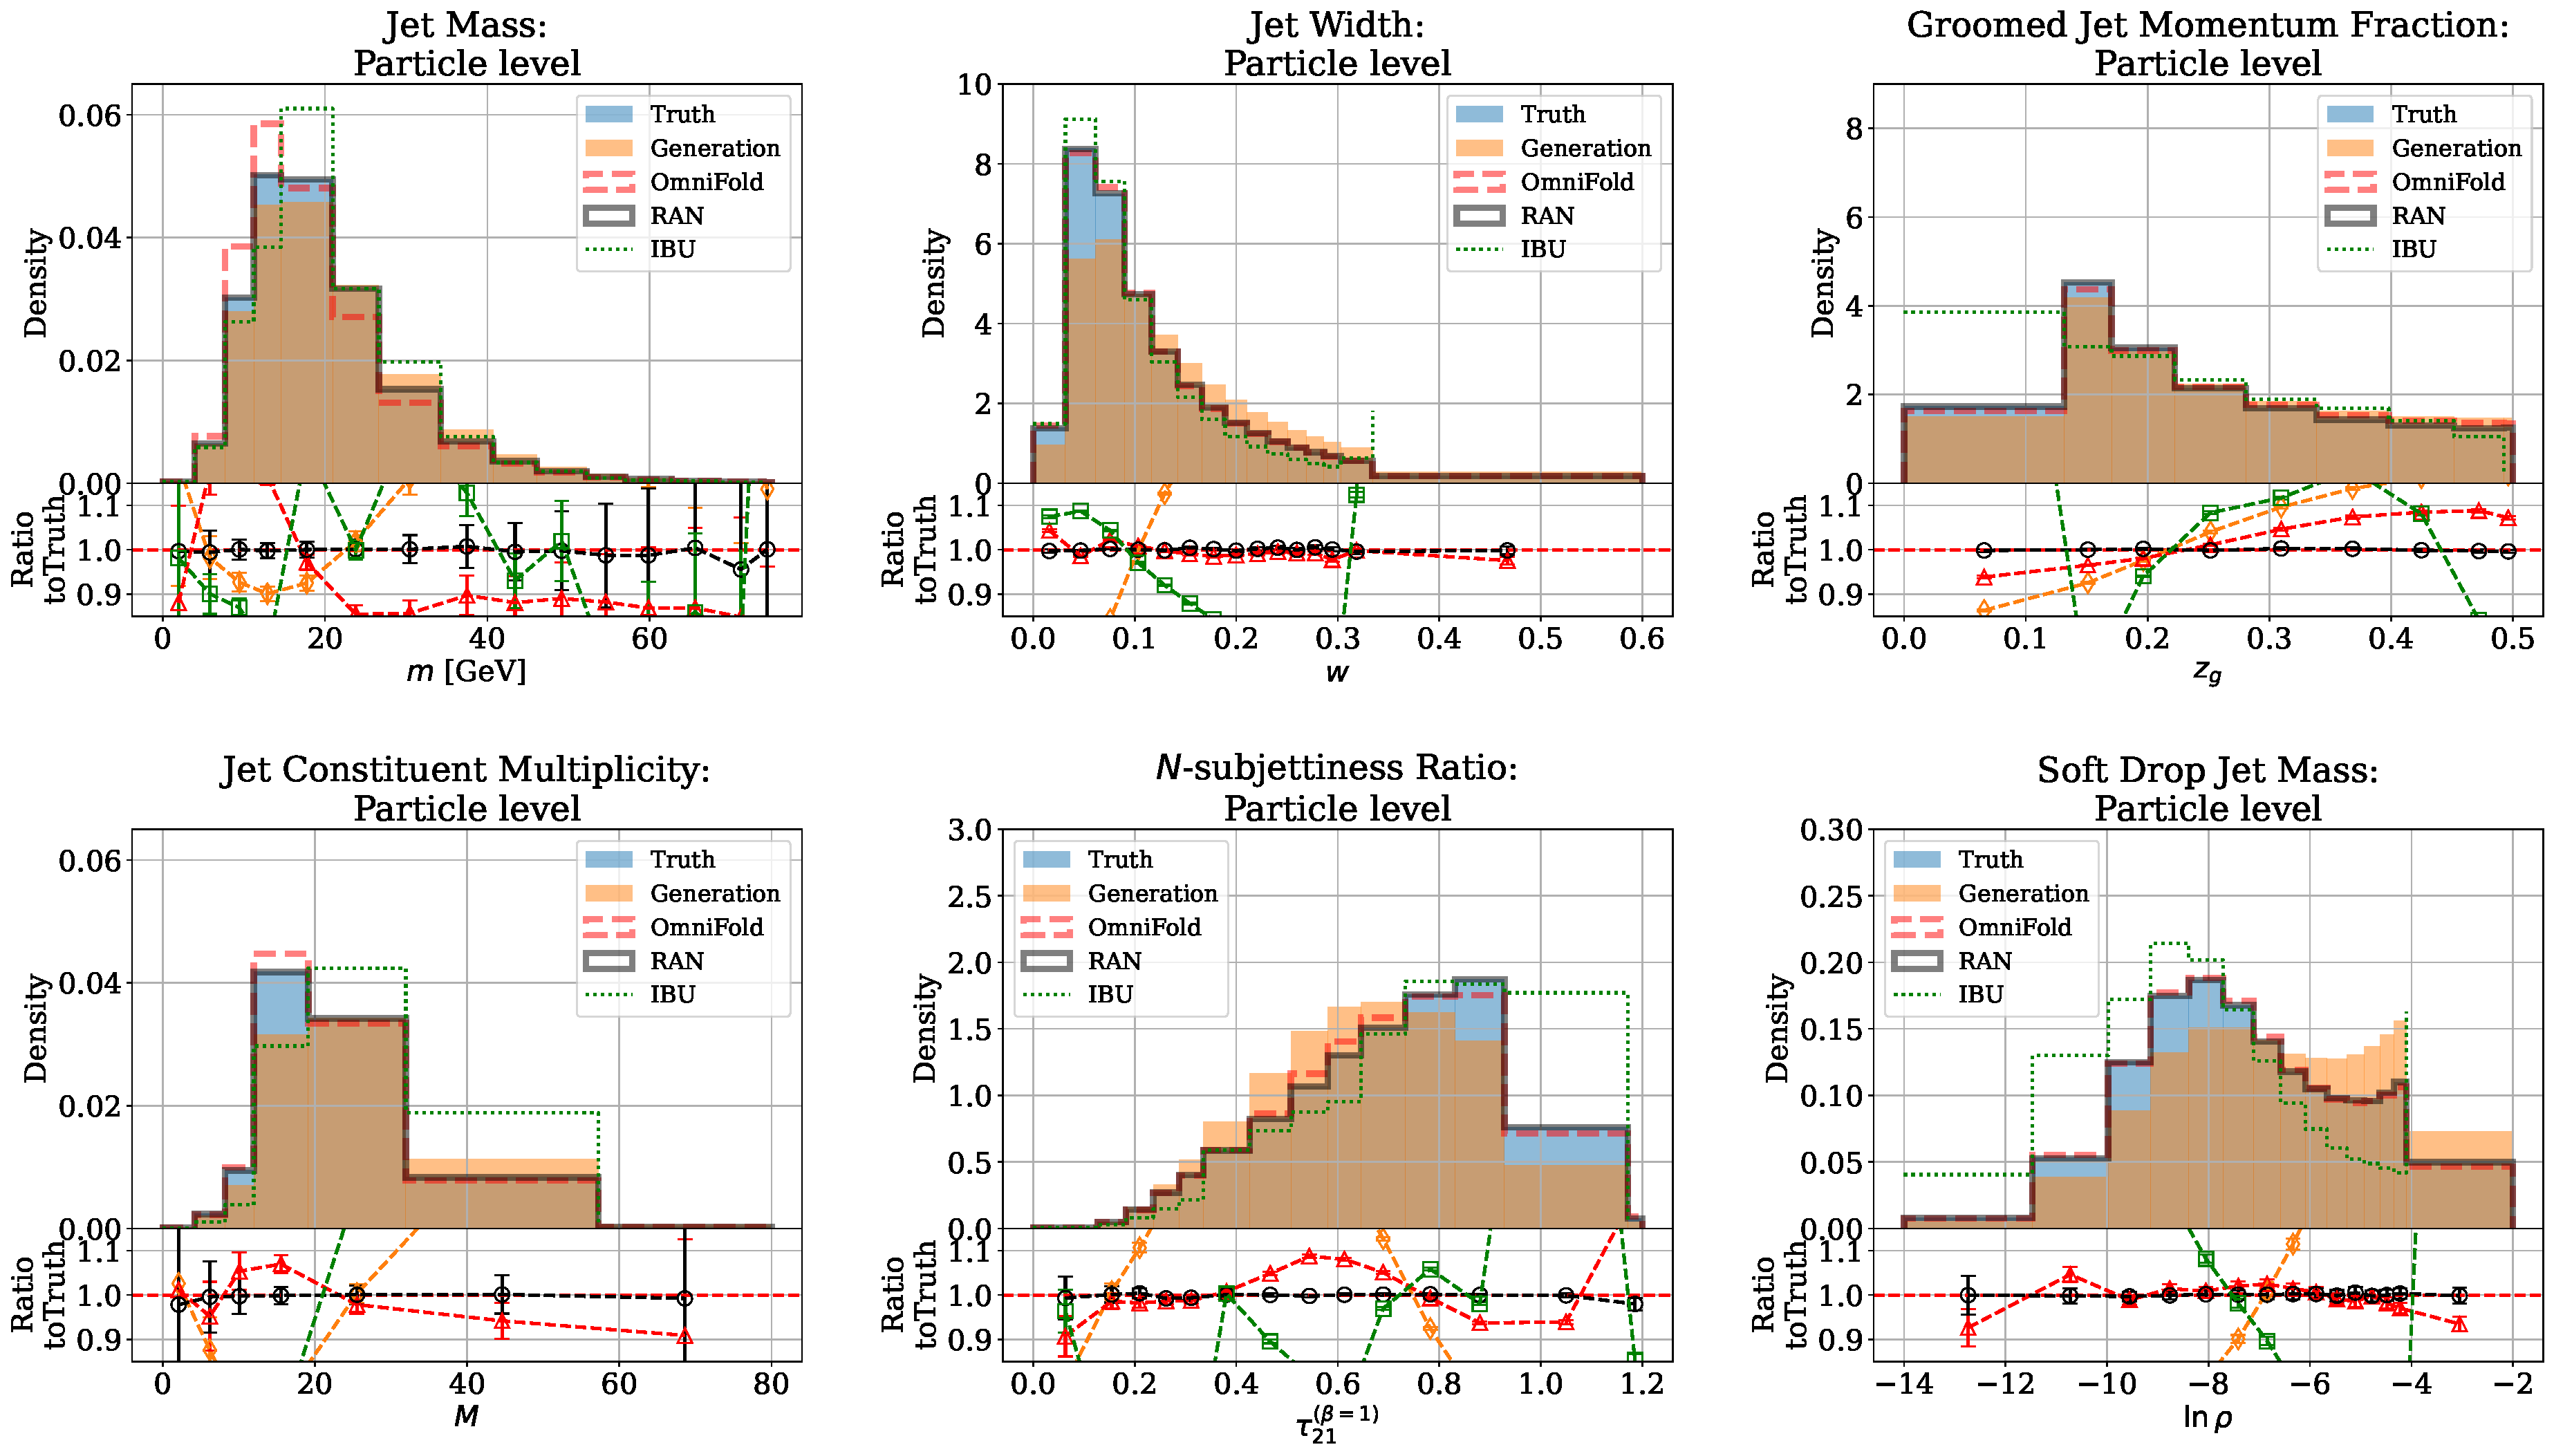
\includegraphics[width = \linewidth]{figures/chapter-06/six_var_with_ratio.pdf}
    \caption[Unfolded particle level distributions for six jet substructure observables, comparing RAN, \textsc{OmniFold}, and IBU.]{Particle level distributions of six jet substructure observables after unfolding. 
    Each panel shows the Truth distribution as the blue filled histogram, the uncorrected Generation as the orange filled histogram, and unfolded results from RAN (black solid), \textsc{OmniFold} (red dashed), and IBU (green dotted). 
    
    The observables span a range of distribution types: jet mass $m$ and soft-drop mass $M$ (left column), constituent multiplicity and jet width $\tau_1$ (middle column), and $N$-subjettiness ratio $\tau_{21}$ and groomed momentum fraction $\ln\rho$ (right column).
    
    The sub--panel under each panel shows the ratio of each unfolded result to truth, demonstrating that RAN achieves close agreement across all observables, particularly in challenging regions such as distribution tails.
    
    Error bars represent the \(1\sigma\) interval computed by training 20 independent runs for each method on the same dataset with different random initialisation.}
    \label{fig:particle-level-distribution}
\end{figure}
            \cref{fig:particle-level-distribution} presents the unfolded particle--level distributions for each of the six jet observables, for RAN, IBU, and \textsc{OmniFold}, compared to the truth distributions.
            %
            Each panel shows the truth spectrum (\textsc{Herwig}, treated as ``Truth'') in filled blue, the generation in filled orange, the unfolded result from RAN as a black solid line, and the unfolded result from \textsc{OmniFold} as a red dashed line, and the result from IBU as a green dotted line.
            %
            The ratio sub--panels below each panel display the unfolded/Truth ratio for each method, indicating how well each method closes the gap to truth across the range of each observable.
            %
            Both RAN and \textsc{OmniFold} achieve good agreement with truth across all observables, a non-trivial accomplishment given the complexity of the distributions, and RAN consistently provides a close match, particularly in regions that are challenging to unfold.
            %
            For example, in the jet mass distribution in \cref{fig:particle-level-distribution}'s, top-left panel, the Generation from \textsc{Pythia} initially undershoots the probability in the high mass tail and misplaces the peak relative to \textsc{Herwig}.
            %
            After unfolding, RAN’s distribution closely follows the truth curve: it accurately reproduces the peak around $m\approx 20$ GeV and the long tail up to high masses. \textsc{OmniFold} also significantly improves the agreement, but its ratio plot reveals a slight residual bias in the tail, with deviations of order 5–10\% from unity in the highest mass bins, whereas RAN’s ratio is within a few percent of unity throughout.
            %
            A similar pattern is seen for the $N$-subjettiness ratio $\tau_{21}$.
            %
            The generator (\textsc{Pythia}) initially produces a broader $\tau_{21}$ distribution than Truth (\textsc{Herwig}), indicating an overestimation of two--prong substructure.
            %
            RAN’s unfolding narrows this distribution to align almost exactly with the truth shape, correcting both the peak and the tail of the $\tau_{21}$ spectrum; \textsc{OmniFold} moves in the right direction but leaves a noticeable difference.
            %
            The \textsc{OmniFold} unfolded $\tau_{21}$ distribution remains slightly too broad, with the ratio to truth dipping below 1.0 in the peak region and rising above 1.0 at higher $\tau_{21}$).
            
            For observables like the jet width $w$ and logarithmic groomed mass $\ln\rho$, which have sharply peaked distributions near zero and long tails, RAN again demonstrates strong performance.
            %
            It captures the steep drop off and the tail behaviour with high fidelity, where \textsc{OmniFold} shows small mismodeling in the intermediate region for $w$ and tail for $\ln\rho$.
            
            The groomed momentum fraction $z_g$ is a particularly challenging variable because of its hard cut-off at $z_g=0.5$.
            %
            Generative or reweighting methods often struggle to reproduce such cut-off behaviour precisely.
            %
            RAN is demonstrated to handle this boundary reasonably well
            %
            The unfolded $z_g$ distribution from RAN matches the truth both in the low $z_g$ region and near the cut-off, correctly recovering the falling slope as $z_g \to 0.5^-$.
            %
            \textsc{OmniFold}’s result for $z_g$ is also quite close to truth with slight undercorrection near the cutoff.
            %
            Finally, the constituent multiplicity $M$. number of particles in the jet. is a particualarly interesting case.
            %
            It is a discrete distribution with a long tail.
            %
            RAN succeeds in reducing the discrepancy at both the low-$M$ and high-$M$ extremes, yielding an unfolded distribution that tracks the truth across the full range.
            %
            \textsc{OmniFold} improves the multiplicity distribution in the bulk region but exhibits larger fluctuations in the very high-multiplicity tail partly due to limited statistics there and the difficulty for the classifier to learn in sparse regions.
            %
            In summary, qualitatively, RAN’s unfolded spectra are virtually indistinguishable from the truth for all six observables, within statistical uncertainties,
            
            The ratio plots in \cref{fig:particle-level-distribution} highlight RAN’s performance. The RAN/Truth ratio is close to 1.0 across the phase space, while the.
            %
            To make these comparisons quantitative, the Wasserstein\(-1\) distances ($W_1$) and VLC divergences between each unfolded distribution and the truth distribution for all methods are computed.
\begin{table}
    \centering
    \def\arraystretch{1.5}
    \begin{tabular}{lcccccc}
        \toprule
        Method & $m$ & $M$ & $w$ & $\tau_{21}$ & $z_g$ & $\ln\rho$ \\
        \midrule
        RAN      & \textbf{3.35} & \textbf{1.19} & \textbf{0.59} & \textbf{0.15} & \textbf{0.80} & \textbf{0.20} \\
        OmniFold & 8.02 & 4.43 & 0.81 & 0.78 & 6.32 & 4.15 \\
        IBU      & 7.40 & 16.07 & 5.28 & 1.52 & 19.18 & 10.31 \\
        \midrule
        Generation & 11.71 & 25.39 & 26.95 & 5.50 & 12.85 & 61.54 \\
        Data       & 33.42 & 71.01 & 181.65 & 60.27 & 97.40 & 378.43 \\
        \bottomrule
    \end{tabular}
    \caption[Wasserstein distances between unfolded and true distributions]{Wasserstein-1 distances ($W_1$) between true distributions for six jet substructure observables and unfolded distributions produced by RAN, OmniFold, and IBU (performed on one dimensional projections onto each observable).
    Values are scaled by $10^{-2}$ for $m$, $M$, and $\tau_{21}$; by $10^{-3}$ for $w$, $z_g$, and $\ln\rho$. 
    RAN achieves the smallest distance for all observables, with particularly dramatic improvements for challenging observables.
    %
    Baseline distances for uncorrected Generation and Data are also shown for reference.}
    \label{tab:comp-w}
\end{table}
\begin{table}
    \centering
    \def\arraystretch{1.5}
    \begin{tabular}{lcccccc}
        \toprule
        Method & $m$ & $M$ & $w$ & $\tau_{21}$ & $z_g$ & $\ln\rho$ \\
        \midrule
        RAN      & \textbf{2.31} & \textbf{5.83} & \textbf{1.29} & \textbf{0.92} & \textbf{0.80} & \textbf{1.27} \\
        OmniFold & 5.06 & 6.32 & 1.33 & 7.91 & 6.84 & 2.34 \\
        IBU      & 5.11 & 16.07 & 7.06 & 17.51 & 11.90 & 3.53 \\
        \midrule
        Generation & 34.92 & 12.89 & 21.86 & 20.33 & 29.17 & 18.86 \\
        Data       & 52.24 & 136.57 & 22.55 & 25.82 & 14.90 & 18.26 \\
        \bottomrule
    \end{tabular}
    \caption[VLC divergence between unfolded and true distributions]{Vincze--Le Cam divergence, $\Delta_{\text{VLC}}$ between true distributions for six jet substructure observables and unfolded distributions produced by RAN, \textsc{OmniFold} and IBU (performed one observable at a time).
    Values are scaled by $10^{-3}$ for $m$, $M$, and $\tau_{21}$; by $10^{-4}$ for $w$, $z_g$, and $\ln\rho$. 
    RAN achieves the smallest divergence for all observables. 
    Baseline divergences for uncorrected Generation and Data are also shown for reference.}
    \label{tab:comp-vlc}
\end{table}
            \cref{tab:comp-w,tab:comp-vlc} summarise these metrics for RAN, \textsc{OmniFold}, and IBU on each jet observable.
            %
            IBU is performed on one dimensional projections onto each jet observable.
            %
            Lower values indicate better agreement with Truth.
            %
            The tables also include, for reference, the baseline distances for the Generation vs. Truth and Data vs. Truth distributions with no unfolding.
            %
            RAN achieves the smallest divergence from Truth under both metrics.
            %
            One also observed that IBU, a binned, per--observable method, generally underperforms the unbinned methods here.
            %
            This is likely due to binning and statistical issues: the need to choose finite bin widths leads to information loss and large uncertainties in sparse regions.
            %
            For $M$, for example, the tail probabilities in high bins were not well estimated, leading to inflated divergence.
            %
            In contrast, RAN and \textsc{OmniFold} operate on unbinned data and can leverage the full event information, yielding superior precision.
            
            It is also noteworthy that RAN’s advantage is achieved while producing a single set of event level weights that simultaneously correct all six distributions.
            %
            In other words, RAN, like \textsc{OmniFold}, inherently unfolds the joint multi--dimensional distribution of these observables without splitting the problem into one dimensional projections
            %
            The fact that a single model can balance all observables and still attain good per observable accuracy is a strong testament to the effectiveness of the adversarial reweighting approach.

            Stability and efficiency, in addition to accuracy, are important considerations for unfolding methods.
            %
            The stability of a RAN's training can probed by performing multiple independent training runs and by bootstrapping subsets of the jet dataset.
            %
            The variations in the resulting unfolded distributions, and in the $W_1$/VLC metrics are found to be small, on the order of a few percent, indicating that the RAN solution is robust to statistical fluctuations and the stochastic nature of training.
            %
            Likewise, \textsc{OmniFold}’s iterative procedure, when run on the same data with different initialisations, converged to comparable results.
            %
            Though minor differences in the weights per iteration can occur, the final distributions were consistent within uncertainties, lending confidence to the RAN's unfolded output.
            %
            IBU, being an analytic iterative method, showed negligible run-to-run variation for fixed binning.
            %
            However, all iterative methods raise the question of convergence and tuning.
            %
            \textsc{OmniFold} requires a subjective choice of a stopping criterion or number of iterations.
            %
            Too few iterations can under correct, too many can overfit the statistical noise.
            %
            IBU similarly depends on a subjective choice of the number of iterations.
            %
            In the \textsc{OmniFold} implementation employed in the studies in this section, five iterations are used, which is the standard approach advocated in~\cite{andreassen_omnifold_2020}, which was sufficient for good performance; using more iterations does not notably improve the agreement and can introduce instability.
            %
            A RAN avoids this ambiguity entirely, since it is trained in one shot to convergence.\footnote{To be clear, a RAN, like any other machine learning based algorithm involves a host of subjective choices, including but not limited to the specific architecture chosen to create the neural networks, to the large array of hyperparameters involved in any neural network training. The point being made here is that iterative ML based methods also require all of these subjective choices, and require the subjective choice of the number of iterations in addition to the other choices.}
            %
            In practice, one finds that RANs train to convergence steadily without signs of overtraining, monitored via the validation loss, and reach a stable solution within a few dozen epochs.
            %
            In terms of computational cost, a RAN’s single--pass adversarial training using the Wasserstein GAN-like setup is comparable to the cost of a one \textsc{OmniFold} iteration.
            %
            But since \textsc{OmniFold} requires two classifier trainings per iteration, and OmniFold was trained for five iterations in these studies, the overall time needed to train a RAN was roughly a fifth of that for \textsc{OmniFold} on these problems.
            %
            IBU is extremely fast for one dimensional histograms, but extending IBU to many dimensions would be combinatorially expensive in terms of computational cost, and practically impossible due to a lack of enough data to fill the bins of high dimensional histograms, whereas RANs and \textsc{OmniFold} scale gracefully to high--dimensional data.
            %
            Thus, a RAN offers an attractive trade--off: it achieves equal or better accuracy than \textsc{OmniFold} on these benchmark tasks, while being simpler to use, since it has no iterative loop to manage, and potentially more efficient.

    \subsubsection{Generality of results}
        Combined with the findings from the Gaussian experiments, these jet experiments suggest that a RAN’s advantages are not specific to a particular distribution but rather reflect general features of the algorithm.
        %
        A RAN’s ability to handle non-overlapping detector effects, demonstrated in the Gaussian toy study, implies it could be helpful in experimental scenarios with poor detector resolutions or acceptance gaps, where traditional unfolding might struggle.
        %
        The jet study confirms that RANs scale to complex, realistic tasks, providing high fidelity unfolding for multiple correlated observables in a single training.
        %
        One expects that these properties would carry over to other unfolding applications.
        %
        For example, measurements of other final states or higher dimensional distributions,\footnote{Such as multivariate phase space distributions.} should similarly benefit from a RAN’s unbinned, non--iterative algorithm.
        %
        Moreover, RAN’s inherently multivariate nature means that, unlike IBU, it can preserve and unfold correlations between observables, an important aspect for modern high--dimensional analyses in particle physics.
        
        Certainly, caution is warranted when extrapolating beyond the tested cases.
        %
        Real experimental data may involve additional complexities in ways not captured by generator differences alone, or require careful treatment of systematic uncertainties in the unfolding procedure.
        %
        Although the RAN performs well on the closure tests described in this section, it remains that case that RANs have only been validated so far using one simulator's output as ``pseudo-data'' and another's as MC, rather than on real experimental measurements.
        
        In summary, the results presented in this section demonstrate that RANs achieve state of the art unfolding performance on both simple and complex tasks.
        %
        They matches or exceed the accuracy of established methods like \textsc{OmniFold} and IBU, while offering improved stability in difficult scenarios and simplified unfolding workflows.
        %
        These characteristics make RANs a promising tool for future precision measurements and exploratory studies in which unfolding high dimensional data without bias is critical.